\documentclass[aps,prd,nofootinbib,superscriptaddress,12pt]{revtex4-2}

\usepackage{graphicx}
\usepackage{hyperref}
\usepackage{amsmath, amssymb}
\usepackage{booktabs}

%% \lb --- a zero-width, hyphen-free breakpoint. Machine-checked statements are
%% cited by their full Lean name, which in a two-column measure is wider than the
%% column and cannot break at all: without a breakpoint those names run into the
%% neighbouring column. A discretionary hyphen would be worse than the overflow,
%% because a reader cannot tell a typeset hyphen from a character of the name.
%% Robust so that it survives a caption's moving argument.
\DeclareRobustCommand{\lb}{\discretionary{}{}{}}

%% D3: PRD long article.
%% Spine: one Seeley-DeWitt coefficient is derived (S2) and then spent (S3-S7);
%% S8 states what the formal layer carries without it; S9 is independent
%% corroboration; S10 is scope. Appendix A is the geometric ground floor.
%% Rendered scalars: papers/D3/tables/*.tex, generated from papers/D3/tables.py.
%% Figures: papers/D3/figures/*.png.

%% ═══════════════════════════════════════════════════════════════════
%% \figuredeferred{id}{reason} — the declared-deferral form
%% ═══════════════════════════════════════════════════════════════════
%%
%% WAVE_EXECUTION_PIPELINE.md §Stage 9: "A figure that is planned but not yet
%% drawn is declared with \figuredeferred{id}{reason}, never omitted silently."
%% The law mandated this form and, measured 2026-08-09, it had ZERO uses across
%% all 21 bundle drafts — nine of which carried no figures at all. Nine bundles
%% with no plan is a charter defect; nine bundles with a *stated* plan and a
%% stated blocker is an honest manuscript in progress, and a referee can tell
%% the two apart only if the plan is on the page.
%%
%% The deferral is DELIBERATELY VISIBLE in the compiled PDF. A silent macro
%% would satisfy `bundle_figure_adequacy` while showing a reader nothing, which
%% is the vacuous-Stage-9 failure ("ALL figures PASS" over an empty set) rebuilt
%% one layer up.
%%
%% ⚠️ The reason must name what BLOCKS the figure, not that it is absent.
%% "not yet drawn" is boilerplate and defeats the purpose; "awaiting the L=8
%% m→0 production run" is a blocker a reader can check and a later pass can
%% discharge.
%%
%% Definition lives here, beside docs/counts.tex, because 21 drafts consume it
%% and a per-draft copy is 21 places for the rendering to drift.

%% Rendered as a non-floating box on purpose. A `figure` float would be subject
%% to revtex's two-column placement rules across eleven drafts for no gain, and
%% a deferral does not need a figure number: it is a promise, not a result.

\providecommand{\figuredeferred}[2]{%
  \par\medskip\noindent
  \fbox{\parbox{0.92\columnwidth}{%
    \small\textbf{Figure deferred: \texttt{#1}.}
    Planned for this section; not yet produced. \emph{Blocked on:} #2.%
  }}%
  \par\medskip
}


\begin{document}

\title{Emergent gravity through black-hole thermodynamics:\\
what one heat-kernel coefficient is forced to do}

\author{John Roehm}

\date{\today}

\begin{abstract}
One Seeley--DeWitt coefficient of the Dirac operator on an
antisymmetric-tetrad-bilinear substrate fixes Newton's constant in the
Sakharov--Adler closed form $G_N = 12\pi/(N_f\Lambda_{\mathrm{UV}}^{2})$, and
the same coefficient stands in the fixed ratio $3/(2\pi)$ to the four-fermion
coupling at which the tetrad condenses, so that no dial separates the induced
gravitational coupling from the condensation threshold. That single number is
then required to supply the linearised and the trace-level Einstein equations,
the post-Newtonian channel ratios, the Bekenstein--Hawking area law, the mass at
which the substrate's black-hole thermodynamics changes branch, the
quadratic-curvature couplings, the Einstein--Cartan torsion amplitude and the
emergent cosmological constant. It clears every published bound we were able to
test except the last. The heat-kernel expansion that delivers $G_N$ also
delivers a positive vacuum energy exceeding the observed one by more than a
hundred orders of magnitude, with no \emph{a priori} cancellation available, so
obtaining the gravitational coupling from matter loops does not shelter a theory
from the cosmological-constant problem. Two alternatives to the condensed-tetrad
route close on numbers the same coefficient produces: a perturbative string-net
route induces a four-fermion coupling three to four orders of magnitude below
the condensation threshold at every cutoff, and the multi-messenger timing of
GW170817 confines the substrate's own vestigial phase to an interval of the
metric-channel susceptibility narrower than its natural range by more than
fourteen orders of magnitude, which is a fine-tuning statement rather than an
exclusion. The subleading logarithm of the horizon entropy is derived from an
$SU(2)_k$ state count rather than fitted, and its coefficient selects the
horizon category, an abelian category being unable to carry the boundary
condition at all. The closure of the calibration on $\alpha_{\mathrm{ADW}} = 1$
rests on structural conditions the substrate records as open, and every identity
below is stated so that it holds whatever value that coefficient takes.
Machine-checked Lean~4 statements are cited by name throughout, with the reach
of each stated wherever it falls short of the classical theorem it is named for.
\end{abstract}

\maketitle

\tableofcontents

%% =====================================================================
%% S1: Introduction
%% =====================================================================
\section{Introduction}
\label{sec:intro}

Induced gravity begins from a reversal: rather than postulating an
Einstein--Hilbert term and quantising it, one integrates matter fields in a
curved background and reads the term off the result~\cite{Sakharov1968,
Adler1980}. The reversal buys a prediction and costs a substrate. The
prediction is that Newton's constant is no longer free, because it is the
coefficient of a one-loop determinant; the cost is that the matter sector, the
cutoff and the composite that plays the role of the frame field all have to be
specified before anything can be computed.

This paper takes that specification to be the antisymmetric fermion bilinear of
Akama, Diakonov and Wetterich~\cite{Akama1978,Diakonov2011}, in which the frame
field is a bilinear in Dirac fields and the spin connection stays an independent
gauge field, and it follows one number through everything the resulting
construction reaches. The number is the Ricci-scalar coefficient $a_2$ of the
Seeley--DeWitt expansion of the squared Dirac operator. Integrated against the
condensed background it delivers
\begin{equation}
\label{eq:intro-sakharov}
G_N^{\mathrm{Sak}}(\Lambda_{\mathrm{UV}}, N_f)
\;=\; \frac{12\pi}{N_f\,\Lambda_{\mathrm{UV}}^{2}},
\end{equation}
and it stands in the fixed ratio $3/(2\pi)$ to the critical four-fermion
coupling $G_c = 8\pi^2/(N_f\Lambda_{\mathrm{UV}}^{2})$ at which the tetrad
condenses in the first place. The pair $(N_f, \Lambda_{\mathrm{UV}})$ is the
whole of the freedom, and \S\ref{sec:substrate} fixes the second of them by
declaring that the measured four-fermion coupling equals the condensation
threshold there. Every quantitative statement in the rest of the paper is a
function of that pair and of nothing else.

The manuscript is organised so that the coefficient is derived before it is
spent. \S\ref{sec:substrate} constructs the substrate, obtains
Eq.~\eqref{eq:intro-sakharov} from the heat-kernel data, and closes on the two
results that the numbers it has just produced decide by themselves: that a
perturbative route to the same four-fermion coupling falls short of the
condensation threshold by three to four orders of magnitude at every cutoff, and
that coarse-graining to a hydrodynamic layer erases the non-Abelian gauge
structure, leaving the gravitational sector as the only place the coefficient
can be tested. \S\ref{sec:efe} through \S\ref{sec:regime} spend it inside that
sector: the field equations and the post-Newtonian channels, the phase of the
substrate that carries a metric but no tetrad, the horizon entropy, and the mass
at which the thermodynamics changes branch. \S\ref{sec:tests} spends it outside
the sector it was calibrated against, in the quadratic-curvature, cosmological
and spin channels. \S\ref{sec:bh-theorems} states what the formal layer carries
without spending the coefficient at all, and says plainly how far that layer
reaches. \S\ref{sec:qcd} reports what the same construction says about the QCD
vacuum, a sector that fixed nothing used earlier. \S\ref{sec:scope} states the
scope of the whole.

Two things should be said before any of that is read, because a referee who
meets them late will re-read what precedes them as overclaiming.

The first is an open hinge. The emergent Newton constant is
$G_N^{\mathrm{emerg}} = \alpha_{\mathrm{ADW}} G_N^{\mathrm{Sak}}$, and every
channel in \S\ref{sec:efe} closes on general relativity exactly at
$\alpha_{\mathrm{ADW}} = 1$. That value is not derived here. What the substrate
records in its place are structural conditions on $\alpha_{\mathrm{ADW}}$ as a
function of the four-fermion coupling, and those conditions fix its limits
rather than its value at any finite coupling; obtaining the value requires the
one-loop graviton two-point function of the broken phase, which is not computed
here. The identities, reductions and biconditionals below are unconditional
algebra in $\alpha_{\mathrm{ADW}}$ and hold whatever it turns out to be. What is
conditional is the physical assertion that the substrate sits at unity, and
\S\ref{sec:efe} states exactly what would settle it.

The second is a convention. Numerals in this paper are quoted at a fiducial
microscopic point, the cutoff at the Planck mass and the Dirac species count at
$N_f = 16$, and that point is a place to evaluate rather than a fit: at
$\alpha_{\mathrm{ADW}} = 1$, matching the observed Newton constant moves the
cutoff by the order-unity factor $\sqrt{12\pi/N_f}$, which is why the paper
treats an order-unity multiple of the Planck mass as the substrate's natural
scale and does not treat the exact Planck value as a prediction. Rendered
quantities are produced from the same code that backs the formal statements, and
they are reported alongside, never in place of, the weaker inequalities the
machine-checked statements actually discharge. Where the two differ, and in the
cosmological-constant channel they differ by twenty-two orders of magnitude,
both are given and the difference is named.

%% =====================================================================
%% S2
%% =====================================================================
\section{The substrate and the coefficient it fixes}
\label{sec:substrate}

One coefficient of the Dirac heat kernel fixes Newton's constant on this
substrate, and no later step introduces a second dial. The substrate is a
system of $N_f$ Dirac species with a four-fermion contact interaction of
strength $G$ and an ultraviolet cutoff $\Lambda_{\mathrm{UV}}$. Above a
critical coupling $G_c = 8\pi^{2}/(N_f\Lambda_{\mathrm{UV}}^{2})$ a tetrad
condenses; integrating the same $N_f$ species against the condensed
background produces an Einstein--Hilbert term whose coefficient is the
Seeley--DeWitt $a_2$ of the Dirac operator. That single coefficient
delivers $G_N = 12\pi/(N_f\Lambda_{\mathrm{UV}}^{2})$, and it stands in a
fixed ratio $3/(2\pi)$ to the very coupling that set the condensation
threshold. Every observable computed later in this manuscript is a
function of the same pair $(N_f,\Lambda_{\mathrm{UV}})$.

Two counts run through the argument and they are not the same number.
$N_f$ is the Dirac species count, a positive real parameter, and it is the
argument taken by the heat-kernel coefficients, by the gap equation and by
Newton's constant; it is the symbol used throughout this section. $N_g$ is
the generation count, a positive integer, and it appears only in the
horizon Witt-invariant sharpening of \S\ref{sec:entropy}. At
Standard-Model content, $N_g$ generations of $16$ Weyl fields each, the two
take the values $N_g = 3$ and $N_f = 24$, both discharged by
\texttt{Sakharov\lb{}Generation\lb{}Bridge.\lb{}sm\_\lb{}counts\_\lb{}differ}. They coincide only in
the degenerate case of two Weyl fields per generation
(\texttt{Sakharov\lb{}Generation\lb{}Bridge.\lb{}counts\_\lb{}agree\_\lb{}iff\_\lb{}two\_\lb{}weyl\_\lb{}per\_\lb{}generation}),
which the Standard Model is not.

\subsection{The tetrad as a fermion bilinear, and the coupling that condenses it}
\label{sec:substrate-gap}

In the Cartan formulation the frame field $e^{A}_{\mu}$ and the spin
connection $\omega^{AB}_{\mu}$ are independent variables. Diakonov replaces
the frame field alone by a bilinear in anticommuting fermion operators,
\begin{equation}
\label{eq:composite-tetrad}
\hat{e}^{A}_{\mu}
= \tfrac{1}{2}\bigl(
\psi^{\dagger}\gamma_{A}\mathcal{D}_{\mu}\psi
- \psi^{\dagger}\overleftarrow{\mathcal{D}}_{\mu}\gamma_{A}\psi\bigr),
\end{equation}
keeping $\omega^{AB}_{\mu}$ as an explicit gauge field so that local Lorentz
invariance is exact at every stage (\cite{Diakonov2011}, Sec.~IV,
Eq.~(11)). The composite-metric route was opened by Akama~\cite{Akama1978},
and Diakonov records that a composite frame field of this type was also
taken up by Wetterich (\cite{Diakonov2011}, Sec.~IV, p.~10); we refer to
the construction as the ADW substrate.

What makes the substrate a four-fermion problem is the index structure of
the invariant volume. The cosmological term
$\int d^{4}x\,\epsilon^{\kappa\lambda\mu\nu}\epsilon_{ABCD}\,
e^{A}_{\kappa}e^{B}_{\lambda}e^{C}_{\mu}e^{D}_{\nu}/4!$
is antisymmetric in both the tangent-space and the spacetime index pairs,
so substituting \eqref{eq:composite-tetrad} makes it quartic in $\psi$ and
quartic in $\psi^{\dagger}$, while the Einstein--Hilbert--Cartan term
becomes quadratic in each (\cite{Diakonov2011}, Secs.~II and V,
Eqs.~(1), (2) and (12)). The quartic term is a contact interaction of
strength $G$ in the tetrad channel, and it is the object a
Hubbard--Stratonovich transformation decouples: one inserts a Gaussian
integral over an auxiliary field carrying the tetrad's index structure,
which trades the quartic vertex for a Yukawa coupling plus a quadratic
penalty $C^{2}/(2G)$, after which the $N_f$ Dirac species are integrated
exactly at one loop.

The result is a self-consistency condition on the tetrad gap $\Delta$. With
a four-dimensional density of states $\rho(p) = c_4\,p^{3}$, where
$c_4 = 1/(4\pi^{2})$ collects the solid angle $S_3/(2\pi)^{4}$ and the
Dirac index trace, the loop integral is
\begin{equation}
\label{eq:gap-integral}
I(\Delta)
= \int_{0}^{\Lambda_{\mathrm{UV}}}\!\frac{\rho(p)}{p^{2}+\Delta^{2}}\,dp
= \frac{c_4}{2}\left[\Lambda_{\mathrm{UV}}^{2}
- \Delta^{2}\ln\!\left(1+\frac{\Lambda_{\mathrm{UV}}^{2}}{\Delta^{2}}\right)\right],
\qquad
I(0) = \frac{\Lambda_{\mathrm{UV}}^{2}}{8\pi^{2}},
\end{equation}
and the gap equation is the fixed-point condition
\begin{equation}
\label{eq:gap-equation}
\Delta = G\,N_f\,\Delta\,I(\Delta).
\end{equation}
$I$ is positive and strictly decreasing on $\Delta \ge 0$
(\texttt{Tetrad\lb{}Gap\lb{}Equation.\lb{}gap\lb{}Integral\_\lb{}pos},
\texttt{Tetrad\lb{}Gap\lb{}Equation.\lb{}gap\lb{}Integral\_\lb{}strict\lb{}Anti}), which fixes the
threshold. Dividing \eqref{eq:gap-equation} by a nonzero $\Delta$ leaves
$G\,N_f\,I(\Delta) = 1$, solvable only when $G\,N_f\,I(0) \ge 1$, so the
critical coupling is
\begin{equation}
\label{eq:critical-coupling}
G_c^{\mathrm{ADW}}(N_f,\Lambda_{\mathrm{UV}})
= \frac{1}{N_f\,I(0)}
= \frac{8\pi^{2}}{N_f\,\Lambda_{\mathrm{UV}}^{2}},
\end{equation}
which is strictly positive for any positive cutoff and species count
(\texttt{ADWMechanism.\lb{}critical\_\lb{}coupling\_\lb{}pos}), and which the gap-integral
route and the effective-potential route agree on
(\texttt{Tetrad\lb{}Gap\lb{}Equation.\lb{}critical\lb{}Coupling\_\lb{}formula},
\texttt{Tetrad\lb{}Gap\lb{}Equation.\lb{}critical\lb{}Coupling\_\lb{}eq\_\lb{}adw}).

The threshold is sharp in both directions. Below it the trivial solution is
the only one: no $\Delta > 0$ satisfies \eqref{eq:gap-equation} when
$G < G_c$, by a contraction argument
(\texttt{Tetrad\lb{}Gap\lb{}Equation.\lb{}gap\_\lb{}trivial\_\lb{}unique\_\lb{}subcritical}). Above it a
nontrivial solution exists, by an intermediate-value argument on the
reduced gap function
(\texttt{Tetrad\lb{}Gap\lb{}Equation.\lb{}gap\_\lb{}nontrivial\_\lb{}exists}), and it is bounded by
the cutoff (\texttt{Tetrad\lb{}Gap\lb{}Equation.\lb{}gap\_\lb{}solution\_\lb{}bounded}) and
increasing in the coupling
(\texttt{Tetrad\lb{}Gap\lb{}Equation.\lb{}gap\_\lb{}solution\_\lb{}monotone}). The transition is a
pitchfork: the curvature of the effective potential at the origin,
$1/G - N_f\Lambda_{\mathrm{UV}}^{2}/(8\pi^{2})$, vanishes exactly at
$G = G_c$ (\texttt{ADWMechanism.\lb{}curvature\_\lb{}zero\_\lb{}at\_\lb{}Gc}), is positive
below and negative above. A leading-order weak-coupling expansion misses
the condensate entirely, which is why the threshold cannot be reached
perturbatively; \S\ref{sec:substrate-wen} makes that quantitative.

Equation~\eqref{eq:critical-coupling} is the operational definition of
$\Lambda_{\mathrm{UV}}$ for everything that follows. It is not an
independently adjustable scale: it is the cutoff at which the measured
four-fermion coupling equals the condensation threshold, and the same
$\Lambda_{\mathrm{UV}}$ is then consumed, without refitting, by Newton's
constant below, by the regime-partition mass, by the entropy's leading
term, by the emergent cosmological constant and by the torsion amplitude.

\subsection{Which phase the substrate occupies}
\label{sec:substrate-phases}

Two order parameters classify the state, and only one combination carries a
tetrad. Writing $C$ for the tetrad expectation value and asking separately
whether the metric bilinear fluctuates, the classification returns the
\emph{pregeometric} phase when $C = 0$ and the bilinear does not fluctuate
(\texttt{ADWMechanism.\lb{}zero\_\lb{}C\_\lb{}no\_\lb{}fluct\_\lb{}gives\_\lb{}pregeometric}), the
\emph{vestigial} phase when $C = 0$ but the bilinear does fluctuate, so
that a metric exists without a tetrad
(\texttt{ADWMechanism.\lb{}zero\_\lb{}C\_\lb{}with\_\lb{}fluct\_\lb{}gives\_\lb{}vestigial}), and the
\emph{full-tetrad} phase whenever $C > 0$, irrespective of the
fluctuations (\texttt{ADWMechanism.\lb{}pos\_\lb{}C\_\lb{}gives\_\lb{}full\_\lb{}tetrad}). A
supercritical gap solution lands in the last of these
(\texttt{Tetrad\lb{}Gap\lb{}Equation.\lb{}gap\_\lb{}implies\_\lb{}full\_\lb{}tetrad}). Classical gravity
requires a tetrad, so the full-tetrad phase is the only candidate;
\S\ref{sec:efe} develops it, and
\S\ref{sec:vestigial} disposes of the vestigial alternative
against the gravitational-wave speed.

\subsection{The heat-kernel coefficient that fixes Newton's constant}
\label{sec:substrate-heat-kernel}

Integrating the $N_f$ Dirac species in the condensed background produces a
gravitational action whose coefficients are the Seeley--DeWitt data of the
Dirac operator $\mathcal{D}$. On a closed four-dimensional Riemannian
manifold,
\begin{equation}
\label{eq:heat-kernel}
\operatorname{Tr}e^{-\tau\mathcal{D}^{2}}
\;\sim\; \sum_{k \ge 0}\tau^{(k-4)/2}\,a_{k}(\mathcal{D}^{2}),
\qquad \tau \to 0^{+},
\end{equation}
where the odd-index coefficients vanish and the even ones are integrals of
local invariants built from the curvature and the endomorphism part of the
operator, carrying an overall normalisation $(4\pi)^{-2}$
(\cite{Vassilevich2003}, Sec.~4.1, statements (1) and (2) and
Eqs.~(4.1), (4.26)--(4.28)). Existence of the asymptotic expansion itself
is a property of the elliptic operator on a spin bundle and is taken here
as an input rather than re-derived.

Three coefficients matter. The leading one is the volume term,
\begin{equation}
\label{eq:a0}
a_{0}(N_f) = \frac{4\,N_f}{(4\pi)^{2}},
\end{equation}
the factor $4$ being the Dirac index trace per species. It is strictly
positive for any positive species count
(\texttt{Heat\lb{}Kernel\lb{}Expansion.\lb{}a0\_\lb{}dirac\_\lb{}pos}) and homogeneous of degree one
in that count, $a_{0}(kN_f) = k\,a_{0}(N_f)$
(\texttt{Heat\lb{}Kernel\lb{}Expansion.\lb{}a0\_\lb{}dirac\_\lb{}linear}); this is the coefficient
that later reproduces the cosmological-constant scale. The second is the
Ricci-scalar coefficient,
\begin{equation}
\label{eq:a2}
a_{2}(x) = a_{2}^{R}(N_f)\,R(x),
\qquad
a_{2}^{R}(N_f) = -\,\frac{N_f}{12\,(4\pi)^{2}},
\end{equation}
whose sign is fixed by the Lichnerowicz form $\mathcal{D}^{2} = -\nabla^{2}
+ R/4 + \dots$ of the squared Dirac operator. It is strictly negative for
positive species count
(\texttt{Heat\lb{}Kernel\lb{}Expansion.\lb{}a2\_\lb{}R\_\lb{}coefficient\_\lb{}neg}), linear in that
count (\texttt{Heat\lb{}Kernel\lb{}Expansion.\lb{}a2\_\lb{}R\_\lb{}coefficient\_\lb{}linear}), and
vanishes exactly when the substrate is empty
(\texttt{Heat\lb{}Kernel\lb{}Expansion.\lb{}a2\_\lb{}R\_\lb{}coefficient\_\lb{}eq\_\lb{}zero\_\lb{}iff}). No other
coefficient carries the Einstein--Hilbert structure, which is what makes
the identification below unique rather than one fit among several.

Integrating the $\Lambda^{2}$-weighted $a_{2}$ term against
$R\sqrt{g}\,d^{4}x$ and matching the Einstein--Hilbert normalisation gives
\begin{equation}
\label{eq:sakharov-closed-form}
\frac{1}{16\pi G_N} = \frac{N_f\,\Lambda_{\mathrm{UV}}^{2}}{12\,(4\pi)^{2}}
= \frac{N_f\,\Lambda_{\mathrm{UV}}^{2}}{192\pi^{2}}
\qquad\Longrightarrow\qquad
G_N^{\mathrm{Sak}} = \frac{12\pi}{N_f\,\Lambda_{\mathrm{UV}}^{2}},
\end{equation}
the Sakharov--Adler closed form of induced
gravity~\cite{Sakharov1968,Adler1980}, here obtained from the $a_{2}$ data
rather than assumed. The identification of the two is
\texttt{Heat\lb{}Kernel\lb{}Expansion.\lb{}G\_\lb{}N\_\lb{}from\_\lb{}a2\_\lb{}eq\_\lb{}G\_\lb{}N\_\lb{}sakharov}, and
positivity for positive cutoff and species count is
\texttt{Linearized\lb{}EFE.\lb{}G\_\lb{}N\_\lb{}sakharov\_\lb{}pos}. Evaluated at the operating
point used throughout this manuscript, with the cutoff at the Planck mass
and the ADW coefficient at unity,
$G_N^{\mathrm{Sak}} = % AUTOGENERATED by scripts/render_paper_tables.py — do not edit by hand.
% Regenerate via `uv run python scripts/render_paper_tables.py` after
% changing any source data or the paper's tables.py SCALARS spec.
% Description: D3 §2: the Sakharov closed form G_N = 12 pi / (N_f Lambda_UV^2) evaluated at the natural point, in GeV^-2.
1.58 \times 10^{-38}%
\unskip\
\mathrm{GeV}^{-2}$.

The coefficient that induces gravity and the coupling that condenses the
tetrad are the same object up to a pure number. Comparing
\eqref{eq:sakharov-closed-form} with \eqref{eq:critical-coupling}, both of
which scale as $1/(N_f\Lambda_{\mathrm{UV}}^{2})$,
\begin{equation}
\label{eq:sakharov-tie}
\frac{G_N^{\mathrm{Sak}}}{G_c^{\mathrm{ADW}}}
= \frac{12\pi}{8\pi^{2}} = \frac{3}{2\pi}
= % AUTOGENERATED by scripts/render_paper_tables.py — do not edit by hand.
% Regenerate via `uv run python scripts/render_paper_tables.py` after
% changing any source data or the paper's tables.py SCALARS spec.
% Description: D3 §2: the ratio G_N^Sak / G_c^ADW as a decimal. The Lean statement gives it in closed form as 3/(2 pi); this is that number, evaluated, as a numerical check that the two definitions agree.
0.477465%
\unskip ,
\end{equation}
so that $G_N^{\mathrm{Sak}} = (3/2\pi)\,G_c^{\mathrm{ADW}}$
(\texttt{Linearized\lb{}EFE.\lb{}G\_\lb{}N\_\lb{}sakharov\_\lb{}eq\_\lb{}ratio\_\lb{}critical\_\lb{}coupling}).
The ratio is a number, not a parameter: it survives any change of $N_f$ or
$\Lambda_{\mathrm{UV}}$, and it is what forbids tuning the induced Newton
constant independently of the condensation threshold. The ADW route carries
one dimensionless coefficient $\alpha_{\mathrm{ADW}}$ relating its emergent
Newton constant to \eqref{eq:sakharov-closed-form}, and demanding that the
two agree fixes it: the heat-kernel constant equals the ADW emergent
constant if and only if $\alpha_{\mathrm{ADW}} = 1$
(\texttt{Heat\lb{}Kernel\lb{}Expansion.\lb{}a2\_\lb{}matches\_\lb{}GNemerg\_\lb{}iff\_\lb{}alpha\_\lb{}ADW\_\lb{}unity}).
That condition is a matching requirement, not a derivation of the one-loop
coefficient; the structural properties that would supply it independently
are stated as hypotheses in \texttt{Linearized\lb{}EFE} and are satisfied by an
explicit ansatz rather than proved from the loop integral.

At the next order the expansion supplies the higher-curvature basis, which
this manuscript states here and spends in \S\ref{sec:tests}. In the
$\{R^{2},\,R_{\mu\nu}R^{\mu\nu},\,R_{\mu\nu\rho\sigma}R^{\mu\nu\rho\sigma}\}$
basis the Dirac $a_{4}$ coefficients are
\begin{equation}
\label{eq:a4-basis}
\bigl(c_{R^{2}},\,c_{\mathrm{Ric}^{2}},\,c_{\mathrm{Riem}^{2}}\bigr)
= \frac{N_f}{12\cdot 180\,(4\pi)^{2}}\,\bigl(-5,\;+7,\;-12\bigr),
\end{equation}
with signs fixed independently of the species count
(\texttt{Heat\lb{}Kernel\lb{}Expansion.\lb{}a4\_\lb{}R\_\lb{}sq\_\lb{}coef\_\lb{}neg},
\texttt{a4\_\lb{}Ricci\_\lb{}sq\_\lb{}coef\_\lb{}pos}, \texttt{a4\_\lb{}Riemann\_\lb{}sq\_\lb{}coef\_\lb{}neg}).
The Gauss--Bonnet combination of these coefficients is
\begin{equation}
\label{eq:a4-gauss-bonnet}
c_{R^{2}} - 4\,c_{\mathrm{Ric}^{2}} + c_{\mathrm{Riem}^{2}}
= -\,\frac{45\,N_f}{12\cdot 180\,(4\pi)^{2}}
= -\,\frac{N_f}{48\,(4\pi)^{2}},
\end{equation}
which is not zero
(\texttt{Heat\lb{}Kernel\lb{}Expansion.\lb{}a4\_\lb{}gauss\_\lb{}bonnet\_\lb{}combination}). The
topological identity is a statement about the integrated density on a
closed four-manifold, not about the local coefficients, and
\eqref{eq:a4-gauss-bonnet} is the local algebra; conflating the two is the
standard way to lose a finite higher-curvature contribution.

\subsection{The perturbative route does not reach the threshold}
\label{sec:substrate-wen}

The obvious alternative to condensing a tetrad is to build gravity
perturbatively on top of an emergent gauge theory, and the natural
candidate is Wen's string-net construction. That construction delivers what
it advertises: from a local bosonic model on a cubic lattice it produces an
emergent $U(1)$ gauge field together with massless Dirac fermions, the
low-energy effective theory being a QED with two families of unit-charge
Dirac fermions (\cite{Wen2003}, Sec.~I.A and Sec.~VII.B). The question is
whether the four-fermion coupling such a route induces can reach
$G_c^{\mathrm{ADW}}$. It is decided entirely by the numbers already in hand.

At one loop the box diagram of an emergent QED with fine-structure constant
$\alpha$ induces a contact coupling
$G_{\mathrm{Wen}} = \alpha^{2}/(4\pi\Lambda_{\mathrm{UV}}^{2})$. Dividing
by \eqref{eq:critical-coupling},
\begin{equation}
\label{eq:wen-ratio}
\frac{G_{\mathrm{Wen}}}{G_c^{\mathrm{ADW}}}
= \frac{\alpha^{2}\,N_f}{32\pi^{3}},
\end{equation}
an identity holding for every nonzero cutoff and every nonzero species
count (\texttt{Emergent\lb{}Gravity\lb{}Bounds.\lb{}wen\_\lb{}adw\_\lb{}ratio\_\lb{}eq}). The cutoff
cancels, so the comparison is not a statement about where one sits in the
ultraviolet; it is a fixed number in $(\alpha, N_f)$. The right-hand side
is increasing in $\alpha$ for $\alpha \ge 0$ and increasing in $N_f$, so a
bound at the upper corner of a parameter window bounds the whole window.
Over $0 \le \alpha \le 1/5$ and $0 < N_f \le 10$ the induced coupling stays
below a thousandth of the threshold for every positive cutoff
(\texttt{Emergent\lb{}Gravity\lb{}Bounds.\lb{}coupling\_\lb{}deficit}).

The bound sharpens by more than half an order of magnitude at a specific
point. At $\alpha = 1/5$ and $N_f = 4$ the deficit factor is
$32\pi^{3}/(\alpha^{2}N_f) = 200\pi^{3}$, and
\begin{equation}
\label{eq:wen-bracket}
\frac{1}{6202} \;<\; \frac{\alpha^{2}N_f}{32\pi^{3}}\biggr|_{\alpha=1/5,\,N_f=4} \;<\; \frac{1}{6201},
\end{equation}
established from rational enclosures of $\pi$ rather than from a
floating-point evaluation
(\texttt{Emergent\lb{}Gravity\lb{}Bounds.\lb{}wen\_\lb{}adw\_\lb{}ratio\_\lb{}bracket}). Combining
\eqref{eq:wen-ratio} and \eqref{eq:wen-bracket} gives the statement in the
form the comparison needs,
$1/6202 < G_{\mathrm{Wen}}/G_c^{\mathrm{ADW}} < 1/6000$, for every nonzero
cutoff (\texttt{Emergent\lb{}Gravity\lb{}Bounds.\lb{}wen\_\lb{}adw\_\lb{}factor\_\lb{}6000}). That last
result is a statement at the fixed point $\alpha = 1/5$, $N_f = 4$,
universally quantified over the cutoff alone; it is not a claim over all
couplings and species counts, and the window-level claim is the weaker
thousandfold bound above.

A perturbative coupling three to four orders of magnitude below the
condensation threshold does not condense a tetrad, and there is no
ultraviolet scale at which it does, because the cutoff has cancelled. The
obstruction is reinforced structurally: what Wen's route supplies is a
one-form $U(1)$, a one-dimensional gauge algebra, while the ADW substrate
requires the six-dimensional $\mathrm{SO}(3,1)$ spin connection of
\eqref{eq:composite-tetrad} as an independent field. Wen's mechanism is
consistent for the photon it was built for, and it cannot be scaled to
gravity by making the coupling larger.

\subsection*{Gauge erasure: why the gravitational sector is the only place this coefficient can be tested}

The substrate is a dissipative many-body system, and its long-wavelength
description is a Schwinger--Keldysh effective field theory of the slow
modes obtained by integrating out the fast ones~\cite{GloriosoLiu2018}.
Coarse-graining to fluid cells is not neutral about which gauge structure
survives it. The one-form symmetry relevant to a hydrodynamic mode is
carried by the centre of the gauge group, and a continuous one-form
symmetry is exactly the case in which the centre is the whole group, that
is, the case in which the group is Abelian
(\texttt{Gauge\lb{}Erasure.\lb{}survives\lb{}Hydro\_\lb{}iff\_\lb{}comm}). For a non-Abelian group
the centre is a proper, discrete subgroup
(\texttt{Gauge\lb{}Erasure.\lb{}not\_\lb{}survives\lb{}Hydro\_\lb{}of\_\lb{}noncomm},
\texttt{Gauge\lb{}Erasure.\lb{}dihedral3\_\lb{}erased}), and breaking a discrete symmetry
produces domain walls rather than Goldstone modes, so the non-Abelian gauge
sector contributes no hydrodynamic mode at all. An Abelian continuous group
does survive, its one-form symmetry photonising into a gapless mode
(\texttt{Gauge\lb{}Erasure.\lb{}circle\_\lb{}survives}). The two cases exhaust the
possibilities: gauge degrees of freedom survive coarse-graining if and only
if the group is Abelian (\texttt{Gauge\lb{}Erasure.\lb{}erasure\_\lb{}dichotomy}).

Applied to the Standard-Model gauge group, $\mathrm{SU}(3)_c$ and
$\mathrm{SU}(2)_L$ are erased and only $U(1)$ survives
(\texttt{Gauge\lb{}Erasure.\lb{}sm\_\lb{}only\_\lb{}u1\_\lb{}survives}). The colour and weak sectors
retain their centre symmetries, which re-enter through the deconfinement
order parameter rather than as fluid modes, so no measurement in those
sectors constrains the substrate's coarse-grained description. The
selection rule is what makes the rest of this manuscript necessary. A
substrate whose non-Abelian structure is invisible below the fluid scale
cannot be tested where the strong and weak interactions are tested; the
$U(1)$ that does survive is the photon and carries no information about the
tetrad channel. The coefficient fixed by \eqref{eq:sakharov-closed-form}
is therefore checkable in exactly one place, the gravitational sector, and
every observable that follows is drawn from it.

%% =====================================================================
%% S3
%% =====================================================================
\section{Einstein's equations on the substrate}
\label{sec:efe}

The substrate reproduces the Einstein equations twice, once in the linearised
sector on a Minkowski background and once at the trace level of the nonlinear
sector, and each reproduction is governed by the same dimensionless number
$\alpha_{\mathrm{ADW}}$ that relates the emergent Newton constant to the
Sakharov--Adler closed form of \S\ref{sec:substrate}. The linearised sector
closes on $\alpha_{\mathrm{ADW}} = 1$, the trace-level nonlinear residual
vanishes if and only if $\alpha_{\mathrm{ADW}} = 1$, the heat-kernel-calibrated
Newton constant agrees with its Sakharov--Adler form if and only if
$\alpha_{\mathrm{ADW}} = 1$, and the post-Newtonian channels agree with general
relativity if and only if $\alpha_{\mathrm{ADW}} = 1$. That a single condition
recurs across channels with independent algebraic content is the structural
result of this section.

One dependency has to be stated before any of it is read. The substrate does
not derive the value of $\alpha_{\mathrm{ADW}}$. What it records instead are
structural conditions on $\alpha_{\mathrm{ADW}}$ as a function of the
four-fermion coupling ratio $x = G/G_c$: strict positivity throughout the broken
phase $x > 1$, collapse to zero as $x \to 1^{+}$, and approach to unity as
$x \to \infty$ (\texttt{Linearized\lb{}EFE.\lb{}H\_\lb{}Vergeles\lb{}Positivity},
\texttt{Linearized\lb{}EFE.\lb{}H\_\lb{}Critical\lb{}Limit\lb{}Collapse},
\texttt{Linearized\lb{}EFE.\lb{}H\_\lb{}Deep\lb{}Gap\lb{}Reduces\lb{}To\lb{}Adler}, collected as
\texttt{Linearized\lb{}EFE.\lb{}H\_\lb{}Vergeles\lb{}NGMode\lb{}Projection}). These are hypotheses, not
theorems, and they are weaker than the condition the section closes on: they fix
the limits of $\alpha_{\mathrm{ADW}}$, not its value at any finite coupling.
Closing them requires the one-loop graviton two-point function of the broken
phase, evaluated at the physical coupling, and that computation is not performed
here and is not available to us from any source we have read. Every closed-form
identity, biconditional and reduction in this section is unconditional algebra
in $\alpha_{\mathrm{ADW}}$ and stands whatever its value turns out to be. What
depends on the open hypotheses is the physical claim that the substrate realises
$\alpha_{\mathrm{ADW}} = 1$, and therefore that it reproduces general relativity
and the observed Newton constant rather than merely admitting a value at which
it would. Right-sign gravity depends on the positivity hypothesis alone: the
sign of $G_N^{\mathrm{emerg}}$ is the sign of $\alpha_{\mathrm{ADW}}$ for
positive cutoff and species count
(\texttt{Linearized\lb{}EFE.\lb{}G\_\lb{}N\_\lb{}emerg\_\lb{}sign}).

\subsection{The emergent Newton constant and its matching locus}
\label{sec:efe-newton}

The emergent Newton constant is the Sakharov--Adler closed form of
\S\ref{sec:substrate} carrying the substrate coefficient,
\begin{equation}
\label{eq:g-n-emerg}
G_N^{\mathrm{emerg}}(\Lambda_{\mathrm{UV}}, N_f, \alpha_{\mathrm{ADW}})
\;=\; \alpha_{\mathrm{ADW}}\, G_N^{\mathrm{Sak}}
\;=\; \alpha_{\mathrm{ADW}}\,\frac{12\pi}{N_f\,\Lambda_{\mathrm{UV}}^{2}}\,,
\end{equation}
so that $\alpha_{\mathrm{ADW}} = 1$ returns the induced-gravity baseline exactly
(\texttt{Linearized\lb{}EFE.\lb{}G\_\lb{}N\_\lb{}emerg\_\lb{}at\_\lb{}alpha\_\lb{}one}) and
$\alpha_{\mathrm{ADW}} = 0$ returns no gravity at all.

Confronting \eqref{eq:g-n-emerg} with a measured Newton constant fixes a locus
rather than a point. For positive cutoff, species count, coefficient and
observed coupling,
\begin{equation}
\label{eq:match-locus}
G_N^{\mathrm{emerg}}(\Lambda_{\mathrm{UV}}, N_f, \alpha_{\mathrm{ADW}})
= G_N^{\mathrm{obs}}
\qquad\Longleftrightarrow\qquad
\Lambda_{\mathrm{UV}}^{2}
\;=\; \frac{12\pi\,\alpha_{\mathrm{ADW}}}{N_f\,G_N^{\mathrm{obs}}}\,,
\end{equation}
which is a biconditional between the physical match and an algebraic condition
on the cutoff (\texttt{Linearized\lb{}EFE.\lb{}G\_\lb{}N\_\lb{}emerg\_\lb{}match\_\lb{}locus}). It is worth
being precise about what \eqref{eq:match-locus} does and does not do: it does
not select $\alpha_{\mathrm{ADW}}$, it trades $\alpha_{\mathrm{ADW}}$ against
$\Lambda_{\mathrm{UV}}$ at fixed $N_f$. Read at $\alpha_{\mathrm{ADW}} = 1$, it
says that the observed Newton constant places the cutoff at
$\Lambda_{\mathrm{UV}} = \sqrt{12\pi/N_f}\,M_{\mathrm{Pl}}$, an order-unity
multiple of the Planck mass for Standard-Model species counts and therefore no
tuning. Read the other way, pinning the cutoff exactly to the Planck mass
$\Lambda_{\mathrm{UV}} = (G_N^{\mathrm{obs}})^{-1/2}$ converts
\eqref{eq:match-locus} into
\begin{equation}
\label{eq:planck-anchor}
G_N^{\mathrm{emerg}}\bigl((G_N^{\mathrm{obs}})^{-1/2}, N_f,
  \alpha_{\mathrm{ADW}}\bigr) = G_N^{\mathrm{obs}}
\qquad\Longleftrightarrow\qquad
12\pi\,\alpha_{\mathrm{ADW}} = N_f
\end{equation}
(\texttt{Linearized\lb{}EFE.\lb{}G\_\lb{}N\_\lb{}emerg\_\lb{}match\_\lb{}at\_\lb{}planck\_\lb{}anchor}). This theorem
transports a hypothesis rather than deriving a result: the choice of anchor is
an input, and what comes out is the value of $\alpha_{\mathrm{ADW}}$ that the
choice forces, namely $N_f/(12\pi)$. That value equals unity only at the
irrational species count $N_f = 12\pi$, so the exact Planck anchor and the
calibration $\alpha_{\mathrm{ADW}} = 1$ are not simultaneously available at
integer $N_f$. The two readings are the same statement seen from two sides, and
we take the first: the calibration is fixed at $\alpha_{\mathrm{ADW}} = 1$ by
the conditions assembled below, and \eqref{eq:match-locus} is then what places
the cutoff. At the natural point the Sakharov--Adler closed form evaluates to
$% AUTOGENERATED by scripts/render_paper_tables.py — do not edit by hand.
% Regenerate via `uv run python scripts/render_paper_tables.py` after
% changing any source data or the paper's tables.py SCALARS spec.
% Description: D3 §2: the Sakharov closed form G_N = 12 pi / (N_f Lambda_UV^2) evaluated at the natural point, in GeV^-2.
1.58 \times 10^{-38}%
\unskip\ \mathrm{GeV}^{-2}$,
exceeding the observed Newton constant by the exact factor $12\pi/N_f$, which
is the same statement as \eqref{eq:planck-anchor}.

\subsection{Linearised equations, trace reversal, and the cosmological reduction}
\label{sec:efe-linear}

In momentum space and de Donder gauge $k^{\mu}\bar{h}_{\mu\nu} = 0$, the
linearised Einstein tensor is purely algebraic in the trace-reversed
perturbation $\bar{h}_{\mu\nu} = h_{\mu\nu} - \tfrac12
\eta_{\mu\nu}\,\mathrm{tr}(h)$, reducing the field equations to
\begin{equation}
\label{eq:linearized}
\Box\,\bar{h}_{\mu\nu} \;=\; -16\pi\,G_N^{\mathrm{emerg}}\,
  T^{\mathrm{matter}}_{\mu\nu}\,,
\qquad
G^{(1)}_{\mu\nu}(k) \;=\; -\tfrac12 k^{2}\,\bar{h}_{\mu\nu}\,.
\end{equation}
Trace reversal is an involution and negates the trace in four dimensions,
$\mathrm{tr}(\bar{h}) = -\,\mathrm{tr}(h)$
(\texttt{Linearized\lb{}EFE.\lb{}trace\_\lb{}reverse\_\lb{}negates\_\lb{}trace},
\texttt{Linearized\lb{}EFE.\lb{}trace\_\lb{}reverse\_\lb{}involutive}), which is what lets the trace
of the linearised Einstein tensor be written back in terms of the untraced
perturbation, $\mathrm{tr}\bigl(G^{(1)}\bigr) = \tfrac12 k^{2}\,\mathrm{tr}(h)$
(\texttt{Linearized\lb{}EFE.\lb{}lin\lb{}Einstein\_\lb{}trace\_\lb{}eq}). The coupling in
\eqref{eq:linearized} is \eqref{eq:g-n-emerg} and nothing else, so every
consequence drawn below inherits the single parameter
$\alpha_{\mathrm{ADW}}$ and no other.

On a homogeneous and isotropic background the same coupling drives the standard
pair. With curvature constant $k$ and scale factor $a$,
\begin{align}
\label{eq:friedmann-i}
H^{2} &\;=\; \frac{8\pi\,G_N^{\mathrm{emerg}}}{3}\,\rho \;-\; \frac{k}{a^{2}}\,,\\
\label{eq:friedmann-ii}
\frac{\ddot a}{a} &\;=\; -\,\frac{4\pi\,G_N^{\mathrm{emerg}}}{3}\,(\rho + 3p)\,,
\end{align}
with the perfect-fluid conservation law $\dot\rho = -3H(\rho + p)$. In the flat
case \eqref{eq:friedmann-i} reduces to $H^{2} = (8\pi
G_N^{\mathrm{emerg}}/3)\rho$ (\texttt{FLRWDynamics.\lb{}hubble\lb{}Squared\_\lb{}flat}), and the
squared Hubble rate driven by the emergent coupling is strictly positive
whenever cutoff, species count, coefficient and density are positive
(\texttt{FLRWDynamics.\lb{}hubble\lb{}Squared\_\lb{}ADW\_\lb{}pos}). This is the point at which the
positivity hypothesis on $\alpha_{\mathrm{ADW}}$ does real work: without it the
substrate admits a wrong-sign emergent coupling and no
Friedmann--Lema\^{i}tre--Robertson--Walker solution at all.

The pair is closed rather than independent. Differentiating
\eqref{eq:friedmann-i} in the flat case and substituting the conservation law
gives $2H\dot H = -8\pi G_N^{\mathrm{emerg}} H(\rho+p)$, from which
$\dot H = -4\pi G_N^{\mathrm{emerg}}(\rho+p)$ follows for $H \neq 0$
(\texttt{FLRWDynamics.\lb{}friedmann\_\lb{}I\_\lb{}dot\_\lb{}eq\_\lb{}conservation\_\lb{}times\_\lb{}coeff},
\texttt{FLRWDynamics.\lb{}acceleration\_\lb{}from\_\lb{}friedmann\_\lb{}I\_\lb{}dot}), and
$\ddot a/a = \dot H + H^{2}$ then returns \eqref{eq:friedmann-ii}. What is
established here is that consistency: given Friedmann I and conservation,
Friedmann II is not an extra assumption. The covariant step behind it, that
$\nabla_{\mu}G^{\mu\nu} = 0$ forces $\nabla_{\mu}T^{\mu\nu} = 0$ and that this
reduces on the cosmological background to the conservation law, is taken from
the standard formulation and is not re-derived on the substrate; the tensor
Einstein equations on a manifold lie outside the present formalisation, which
works with the linearised sector, the trace, and this reduction.

\subsection{The nonlinear equations at trace level}
\label{sec:efe-nonlinear}

Varying the Seeley--DeWitt effective action of \S\ref{sec:substrate} with
respect to the tetrad and contracting with the inverse metric gives a scalar
equation. Under the substrate rescaling the emergent stress-energy trace is
$T^{\mu}{}_{\mu,\,\mathrm{emerg}} = \alpha_{\mathrm{ADW}}\,\rho$, so it
coincides with the bare matter trace exactly at the calibration value, for any
non-vanishing source
(\texttt{Nonlinear\lb{}EFE.\lb{}emergent\lb{}Stress\lb{}Energy\lb{}Trace\_\lb{}eq\_\lb{}matter\_\lb{}iff\_\lb{}alpha\_\lb{}unity}).
Writing the trace equation about the configuration in which Einstein and matter
balance at $\alpha_{\mathrm{ADW}} = 1$ leaves the residual
\begin{equation}
\label{eq:efe-residual}
\mathcal{R}_{\mathrm{trace}}(G_N, \rho, \alpha_{\mathrm{ADW}})
\;=\; 8\pi\,G_N\,\rho\,(\alpha_{\mathrm{ADW}} - 1)\,,
\end{equation}
and for positive Newton constant and non-vanishing source this residual
vanishes if and only if $\alpha_{\mathrm{ADW}} = 1$
(\texttt{Nonlinear\lb{}EFE.\lb{}efe\lb{}Residual\lb{}Trace\_\lb{}eq\_\lb{}zero\_\lb{}iff\_\lb{}alpha\_\lb{}unity}). The
converse direction is the one with content: any $\alpha_{\mathrm{ADW}} \neq 1$
leaves a residual linear in $\alpha_{\mathrm{ADW}} - 1$ and proportional to the
source, which is the deviation channel the observational tests of
\S\ref{sec:efe-ppn} probe. Evaluated at the emergent coupling itself, the
statement becomes a falsifier: for positive cutoff, species count and
coefficient and non-vanishing source, every $\alpha_{\mathrm{ADW}} \neq 1$
violates the substrate's nonlinear field equations
(\texttt{Nonlinear\lb{}EFE.\lb{}perturbed\_\lb{}alpha\_\lb{}not\_\lb{}H\_\lb{}Nonlinear\lb{}EFEHolds}).

Two scope statements belong with \eqref{eq:efe-residual}. It is the trace of the
field equations, not the full tensor system; the trace carries the
Newton-constant calibration, the emergent-versus-matter source comparison and
the post-Newtonian deviations, and it does not carry the tensor structure, which
the present formalisation does not construct. And the higher-curvature terms
generated at the same order in the heat-kernel expansion are retained rather
than dropped: their trace-level contribution inherits the bound established for
the individual Seeley--DeWitt coefficients, so it does not disturb the residual
\eqref{eq:efe-residual} at the orders at issue
(\texttt{Nonlinear\lb{}EFE.\lb{}higher\lb{}Curvature\lb{}Correction\_\lb{}abs\_\lb{}bound}).

\subsection{Post-Newtonian channels collapse onto one parameter}
\label{sec:efe-ppn}

At linearised post-Newtonian order the substrate makes predictions in channels
that the parametrised post-Newtonian framework treats separately. The
deflection and ringdown channels enter through the emergent coupling alone and
rescale linearly with it; the perihelion channel enters through the standard
post-Newtonian combination $(2 + 2\gamma - \beta)/3$ with $\gamma =
\alpha_{\mathrm{ADW}}$ and $\beta = 1$. Relative to their general-relativistic
values the channel ratios are therefore
\begin{equation}
\label{eq:ppn-triple}
\bigl(\alpha_{\mathrm{deflect}},\ \alpha_{\mathrm{precess}},\
      \alpha_{\mathrm{ringdown}}\bigr)
\;=\;
\Bigl(\alpha_{\mathrm{ADW}},\ \tfrac{2\alpha_{\mathrm{ADW}}+1}{3},\
      \alpha_{\mathrm{ADW}}\Bigr)\,,
\end{equation}
a one-parameter family. Every channel returns unity at
$\alpha_{\mathrm{ADW}} = 1$, and the perihelion channel returns unity only
there, since the coefficient $2/3$ makes
$(2\alpha_{\mathrm{ADW}}+1)/3 = 1$ a genuine linear equation rather than an
identity (\texttt{Nonlinear\lb{}EFE.\lb{}precession\lb{}Ratio\_\lb{}eq\_\lb{}one\_\lb{}iff\_\lb{}alpha\_\lb{}unity}).

The comparison that makes this a prediction is with the framework the
measurements are normally reported in. There the post-Newtonian metric carries
ten parameters, of which $\gamma$ and $\beta$ are the only ones non-vanishing in
general relativity and in scalar-tensor gravity, and a theory based on an
invariant action principle retains several of the others as free
(Will, \emph{Living Rev.\ Relativity} \textbf{17}, 4 (2014)~\cite{Will2014},
\S3.2 and Table~2). Light deflection is controlled by $\gamma$ alone, through
the factor $\tfrac12(1+\gamma)$ of \S4.1.1, Eq.~(59); the perihelion advance is
controlled by the combination $(2+2\gamma-\beta)/3$ of \S4.2, Eq.~(64). The two
solar-system channels therefore move with two parameters that the framework
leaves independent, and the ringdown frequency is not a post-Newtonian
observable at all, so it is not fixed by $\gamma$ and $\beta$ in any case.

The substrate has no such freedom, and this is what is falsifiable about it.
Because \eqref{eq:ppn-triple} is a single-parameter family, the relations among
the channels carry no adjustable content at all: the ringdown ratio must equal
the deflection ratio exactly, and the perihelion deviation must be two-thirds of
the deflection deviation,
\begin{equation}
\label{eq:ppn-cross-channel}
\alpha_{\mathrm{precess}} - 1
\;=\; \tfrac{2}{3}\,\bigl(\alpha_{\mathrm{deflect}} - 1\bigr)
\end{equation}
(\texttt{Nonlinear\lb{}EFE.\lb{}precession\_\lb{}dev\_\lb{}eq\_\lb{}two\_\lb{}thirds\_\lb{}deflection\_\lb{}dev}). No
choice of $\alpha_{\mathrm{ADW}}$ restores agreement with a measurement that
violates \eqref{eq:ppn-cross-channel}, because $\alpha_{\mathrm{ADW}}$ has
already been eliminated between the channels. That is the difference between a
prediction and a fit: a fit has a parameter left to move, and here there is
none. A campaign that measured deflection and perihelion deviations in any other
proportion would falsify the construction without ever determining
$\alpha_{\mathrm{ADW}}$. The deviations themselves are within reach of existing
sensitivity rather than hypothetical: very-long-baseline interferometry
determines $\gamma - 1$ at the level of parts in $10^{4}$~\cite{Will2014},
\S4.1.1, and any $|\alpha_{\mathrm{ADW}} - 1|$ exceeding $3 \times 10^{-4}$
produces a deflection deviation above that floor
(\texttt{Nonlinear\lb{}EFE.\lb{}deflection\lb{}Ratio\_\lb{}deviation\_\lb{}exceeds\_\lb{}VLBI\_\lb{}floor}). Solar-system
deflection has agreed with general relativity since the 1919 eclipse
measurements~\cite{Eddington1919} and now agrees at that precision, so the
observational input the substrate consumes is $\alpha_{\mathrm{ADW}} = 1$ to
within parts in $10^{4}$.

\subsection{One condition, several independent channels}
\label{sec:efe-recurrence}

The calibration of \S\ref{sec:substrate} closes on the same value. The Newton
constant read off the $a_2$ Seeley--DeWitt coefficient of the Dirac operator
coincides with the substrate's emergent Newton constant \eqref{eq:g-n-emerg} if
and only if $\alpha_{\mathrm{ADW}} = 1$, exactly and with no tolerance, for any
positive cutoff and species count
(\texttt{Heat\lb{}Kernel\lb{}Expansion.\lb{}a2\_\lb{}matches\_\lb{}GNemerg\_\lb{}iff\_\lb{}alpha\_\lb{}ADW\_\lb{}unity}),
the two closed forms being equal as functions of $(\Lambda_{\mathrm{UV}}, N_f)$
(\texttt{Heat\lb{}Kernel\lb{}Expansion.\lb{}G\_\lb{}N\_\lb{}from\_\lb{}a2\_\lb{}eq\_\lb{}G\_\lb{}N\_\lb{}sakharov}).

It is worth saying plainly what the recurrence is and is not. Taken one at a
time these biconditionals are elementary: the emergent Newton constant is
defined as $\alpha_{\mathrm{ADW}}$ times the Sakharov--Adler form, so its
agreement with that form at $\alpha_{\mathrm{ADW}} = 1$ is close to a
restatement. The content lies in the fact that the same $\alpha_{\mathrm{ADW}}$
appears in each place it could have appeared independently. It sets the
normalisation of the induced Einstein--Hilbert term against the heat-kernel
coefficient; it sets the ratio of emergent to bare stress-energy trace; it sets
the coupling in the cosmological reduction; and it sets the post-Newtonian
channel ratios. A construction in which these were separate coefficients would
have as many free numbers as channels, and each measurement would fix one of
them. Here a measurement in any channel fixes all of them, and every channel
already measured points at the same value.

\subsection{What remains open, and what it would take to close it}
\label{sec:efe-open}

The condition $\alpha_{\mathrm{ADW}} = 1$ is not derived on the substrate. The
conditions recorded in its place are limits, and they leave the interior of the
broken phase undetermined: positivity for $x = G/G_c > 1$, collapse
$\alpha_{\mathrm{ADW}} \to 0$ as $x \to 1^{+}$, and
$\alpha_{\mathrm{ADW}} \to 1$ as $x \to \infty$. They are not vacuous. The
constant function $0$ fails the deep-gap limit, the constant function $1$ fails
the critical-limit collapse, and a sign-reversed interpolation fails positivity
(\texttt{Linearized\lb{}EFE.\lb{}vergeles\_\lb{}fails\_\lb{}at\_\lb{}constant\_\lb{}zero},
\texttt{Linearized\lb{}EFE.\lb{}vergeles\_\lb{}fails\_\lb{}at\_\lb{}constant\_\lb{}one},
\texttt{Linearized\lb{}EFE.\lb{}vergeles\_\lb{}fails\_\lb{}at\_\lb{}negated\_\lb{}linear}), and they are
jointly satisfiable, the interpolation $\alpha_{\mathrm{ADW}}(x) = 1 - 1/x$
meeting all of them
(\texttt{Linearized\lb{}EFE.\lb{}alpha\lb{}ADW\_\lb{}linear\_\lb{}satisfies\_\lb{}vergeles}). That
interpolation is an illustration of consistency and not a derivation of the
coefficient, and it makes the gap concrete: it attains
$\alpha_{\mathrm{ADW}} = 1$ only asymptotically, so on that reading the
calibration value is a boundary value the theory approaches deep in the broken
phase rather than one it takes at a finite coupling.

Two things would close the gap, and neither is supplied here. The first is the
one-loop graviton two-point function of the broken phase, computed at the
physical coupling, which is what actually returns a number for
$\alpha_{\mathrm{ADW}}$; the framework needed to set it up is in place in the
lattice and continuum treatments of composite-tetrad gravity
\cite{Akama1978, Diakonov2011}, and the extraction of the prefactor is the step
that is missing. The second is the removal of the standing restriction on the
lattice regularisation's unitarity. Unitarity of the time-evolution operator of
four-dimensional lattice gravity in Minkowski signature is established in
Vergeles~\cite{Vergeles2025}, whose \S IV.A, Statement~3 proves that the
evolution is unitary and preserves the number of degrees of freedom, and whose
\S II.B, Eqs.~(2.27)--(2.29) identifies the long-wave limit of the lattice
action as the Einstein--Cartan--Palatini action minimally coupled to the Dirac
field. That result is explicitly restricted, in its own abstract and again in
\S V.1, to lattices conserving the number of degrees of freedom: extending it to
evolution that changes that number requires an identity, Eq.~(5.7) there, which
that work states it does not know how to prove and is not certain is
well posed. The positivity condition on $\alpha_{\mathrm{ADW}}$ is motivated by
that unitarity result but is not derived in it, and we record it as a hypothesis
for exactly that reason.

None of the identities, reductions or biconditionals above is conditioned on any
of this. \eqref{eq:g-n-emerg} through \eqref{eq:ppn-cross-channel} hold for
every value of $\alpha_{\mathrm{ADW}}$, and each biconditional is an exact
statement about which value makes a given channel close. What is conditional is
the physical assertion that the substrate sits at that value. Read as a
conditional prediction the section is unaffected by the gap: if the substrate
realises $\alpha_{\mathrm{ADW}} = 1$ then it reproduces the Einstein equations
in both sectors, the observed Newton constant on the locus
\eqref{eq:match-locus}, the cosmological dynamics
\eqref{eq:friedmann-i}--\eqref{eq:friedmann-ii}, and general relativity in every
post-Newtonian channel; and if it does not, the residual
\eqref{eq:efe-residual} and the cross-channel relation
\eqref{eq:ppn-cross-channel} say exactly where the failure shows up.

%% =====================================================================
%% S4
%% =====================================================================
\section{The vestigial mode is confined, not excluded}
\label{sec:vestigial}

The tetrad channel of \S\ref{sec:efe} does not condense in a single step.
Between the disordered vacuum and the condensed tetrad lies an
intermediate branch in which a metric already exists as a fermion
bilinear while the tetrad expectation still vanishes. This section
develops that branch, derives the propagation speed it would assign to a
spin-two disturbance, and confronts that speed with the multi-messenger
timing of GW170817. The outcome is a constraint rather than an exclusion.
The datum admits the branch, and admits it only on an interval of the
metric-channel susceptibility that lies strictly inside the range
naturalness allows and is narrower than that range by more than a factor
of $10^{14}$.

\subsection{The trichotomy of tetrad condensation}
\label{sec:vestigial-trichotomy}

Take the tetrad to be the expectation of an antisymmetric fermion
bilinear, $e^a_\mu = \langle \hat E^a_\mu \rangle$, and the metric to be
the corresponding bilinear correlator
\begin{equation}
\label{eq:metric-bilinear}
g_{\mu\nu} \;=\; \eta_{ab}\,\bigl\langle \hat E^a_\mu\, \hat E^b_\nu
\bigr\rangle ,
\end{equation}
\noindent
which is the Akama--Diakonov--Wetterich construction in the form Volovik
writes it (\S III, Eqs.~(18) and (19) of
Ref.~\cite{Volovik2024Vestigial}). The tetrad condensate amplitude $C$ of
the gap equation and the fluctuation of the metric channel are then
independent order parameters, and which branch the vacuum occupies is
fixed by which of them is switched on.

With $C = 0$ and the metric channel unexcited, neither
Eq.~\eqref{eq:metric-bilinear} nor the tetrad has support and the vacuum
is pregeometric
(\texttt{ADWMechanism.\lb{}zero\_\lb{}C\_\lb{}no\_\lb{}fluct\_\lb{}gives\_\lb{}pregeometric}). With
$C = 0$ but the metric channel excited, the correlator
\eqref{eq:metric-bilinear} is nonzero while $e^a_\mu$ still vanishes, and
the vacuum is vestigial
(\texttt{ADWMechanism.\lb{}zero\_\lb{}C\_\lb{}with\_\lb{}fluct\_\lb{}gives\_\lb{}vestigial}). For
$C > 0$ the tetrad itself condenses, and it does so for either state of
the metric channel (\texttt{ADWMechanism.\lb{}pos\_\lb{}C\_\lb{}gives\_\lb{}full\_\lb{}tetrad}).
Volovik states the resulting sequence as
$\text{disorder} \to \text{GR} \to \text{ECSK}$ (Eq.~(20) of
Ref.~\cite{Volovik2024Vestigial}).

The middle branch is the one this section is about. It carries metric
structure and no tetrad
(\texttt{Vestigial\lb{}Gravity.\lb{}vestigial\_\lb{}has\_\lb{}metric\_\lb{}no\_\lb{}tetrad}), and that
asymmetry is observable. Bosonic matter couples to the full metric
\eqref{eq:metric-bilinear} and propagates on it; a fermion needs a
vierbein to convert its spinor index into a spacetime index, and in the
vestigial branch there is none to convert it with. Volovik draws the
consequence directly: fermions interact with the tetradic part of the
metric while bosons interact with the full metric, so a boson and a
fermion released in the same gravitational field do not follow the same
trajectory (\S III, following Eqs.~(21) and (22) of
Ref.~\cite{Volovik2024Vestigial}). Formally, the coupling seen by bosons
and the coupling seen by fermions differ in the vestigial branch and
coincide in the full-tetrad branch
(\texttt{Vestigial\lb{}Gravity.\lb{}wep\_\lb{}distinguishes\_\lb{}vestigial\_\lb{}from\_\lb{}full}), a
nonvanishing tetrad expectation occurs in the full-tetrad branch alone
(\texttt{Vestigial\lb{}Gravity.\lb{}tetrad\_\lb{}only\_\lb{}in\_\lb{}full}), and the equivalence
principle holds there and nowhere else
(\texttt{Vestigial\lb{}Gravity.\lb{}ep\_\lb{}only\_\lb{}in\_\lb{}full\_\lb{}tetrad}). The weak
equivalence principle is therefore the observable that separates the
vestigial branch from the full-tetrad branch, and the classical gravity
assembled in \S\ref{sec:efe} is available on the full-tetrad branch only.

\subsection{The speed a vestigial mode would propagate at}
\label{sec:vestigial-speed}

Identifying the vestigial metric-channel excitation with a propagating
spin-two disturbance gives, at leading order,
\begin{equation}
\label{eq:c-gw}
c_{\mathrm{GW}}(\chi_{\mathrm{vest}}) \;=\;
c\,\sqrt{\chi_{\mathrm{vest}}} ,
\end{equation}
\noindent
where $\chi_{\mathrm{vest}}$ is the dimensionless susceptibility of the
metric channel of Eq.~\eqref{eq:metric-bilinear}.

Equation~\eqref{eq:c-gw} belongs to the present construction rather than
to the identification it borrows. It is the transplantation that
introduces the susceptibility: the identification of a vestigial
second-sound mode with a graviton was advanced on a de~Sitter two-fluid
background, whereas here the mode rides on the antisymmetric tetrad
bilinear of \S\ref{sec:efe}, whose metric channel carries a
susceptibility the substrate does not determine. Throughout this section
$\chi_{\mathrm{vest}}$ is a free parameter and nothing below computes it.
At $\chi_{\mathrm{vest}} = 1$, Eq.~\eqref{eq:c-gw} returns
$c_{\mathrm{GW}} = c$ exactly
(\texttt{Gravitational\lb{}Waves.\lb{}c\_\lb{}GW\_\lb{}at\_\lb{}chi\_\lb{}one}), so any identification
whose mode speed is already fixed to $c$ sits at that anchor and is
untouched by the bound derived below. What the bound acts on is the
freedom this work introduced.

Write the fractional offset as
$\delta(\chi_{\mathrm{vest}}) = \sqrt{\chi_{\mathrm{vest}}} - 1$. Three
properties of $\delta$ carry the argument. It vanishes exactly and only
at the anchor: for $\chi_{\mathrm{vest}} \ge 0$,
$\delta(\chi_{\mathrm{vest}}) = 0$ if and only if
$\chi_{\mathrm{vest}} = 1$, as a biconditional
(\texttt{Gravitational\lb{}Waves.\lb{}c\_\lb{}GW\_\lb{}deviation\_\lb{}zero\_\lb{}iff\_\lb{}chi\_\lb{}one}), so
agreement with general relativity at this order is not a regime but a
point. It is the measured quantity for every choice of the light speed,
since
$\bigl(c_{\mathrm{GW}}(\chi_{\mathrm{vest}},c) - c\bigr)/c
= \delta(\chi_{\mathrm{vest}})$ for every $c \neq 0$
(\texttt{Gravitational\lb{}Waves.\lb{}c\_\lb{}GW\_\lb{}relative\_\lb{}deviation\_\lb{}eq}), which is
what makes the constraint below independent of any rescaling of $c$. And
it is strictly increasing in $\chi_{\mathrm{vest}}$ on the non-negative
susceptibilities
(\texttt{Gravitational\lb{}Waves.\lb{}c\_\lb{}GW\_\lb{}deviation\_\lb{}strict\_\lb{}mono}), so a bound
on the signed offset inverts to an interval in $\chi_{\mathrm{vest}}$
with no ambiguity.

\subsection{The GW170817 cap and the interval it leaves}
\label{sec:vestigial-ligo}

The joint observation of GW170817 and GRB~170817A gives an arrival-time
offset of $(+1.74 \pm 0.05)\,\mathrm{s}$ over a luminosity distance of
$26\,\mathrm{Mpc}$, which the LIGO--Virgo collaboration converts into the
asymmetric bound
$-3\times 10^{-15} \le \Delta v/v_{\mathrm{EM}} \le +7 \times 10^{-16}$
on the fractional difference between the speed of gravity and the speed
of light (\S4.1, Eq.~(1) of Ref.~\cite{Abbott2017GW170817}). We adopt
throughout the conservative symmetric envelope
$|\Delta c/c| \le % AUTOGENERATED by scripts/render_paper_tables.py — do not edit by hand.
% Regenerate via `uv run python scripts/render_paper_tables.py` after
% changing any source data or the paper's tables.py SCALARS spec.
% Description: D3 §4: the GW170817 two-sided fractional cap on the gravitational-wave propagation speed, as stored in constants.py.
3 \times 10^{-15}%
\unskip$,
which is the looser of its two sides.

The naturalness window on the susceptibility runs from
$\chi_{\mathrm{vest}} = \input{tables/chi_vest_natural_lower.tex}\unskip$
to
$\chi_{\mathrm{vest}} = % AUTOGENERATED by scripts/render_paper_tables.py — do not edit by hand.
% Regenerate via `uv run python scripts/render_paper_tables.py` after
% changing any source data or the paper's tables.py SCALARS spec.
% Description: D3 §4: the upper endpoint of the natural chi_vest range.
10%
\unskip$,
one decade on either side of the unit-normalised bubble-integral scale.
This is a prior adopted by the present work, on the same convention as
the $\alpha_{\mathrm{ADW}}$ window of \S\ref{sec:efe}, and not a
published derivation. Its lower edge marks the critical-fluid regime in
which the susceptibility of the vestigial condensate is still
well-defined, its upper edge the strong-coupling regime beyond which the
one-loop expansion of \S\ref{sec:efe} fails.

Both endpoints of that window fail the cap, and fail it by a wide margin:
the offsets there are of order unity, against a cap of order
$10^{-15}$. Each endpoint is discharged separately
(\texttt{Gravitational\lb{}Waves.\lb{}natural\_\lb{}lower\_\lb{}violates\_\lb{}ligo} and
\texttt{Gravitational\lb{}Waves.\lb{}natural\_\lb{}upper\_\lb{}violates\_\lb{}ligo}) and the pair
is bundled as the statement that no susceptibility equal to either
endpoint satisfies the cap
(\texttt{Gravitational\lb{}Waves.\lb{}natural\_\lb{}endpoints\_\lb{}violate\_\lb{}ligo\_\lb{}window}).
Because the fractional offset is the same for every nonzero $c$, no
rescaling of the light speed rescues either endpoint
(\texttt{Gravitational\lb{}Waves.\lb{}natural\_\lb{}endpoints\_\lb{}violate\_\lb{}ligo\_\lb{}for\_\lb{}every\_\lb{}c}).
These are statements about the endpoints. They say nothing about the
interior, and reading them as an exclusion of the window would be an
error of quantification.

The interior is settled by the positive half of the result. For
$\chi_{\mathrm{vest}} \ge 0$ whose offset satisfies the cap, with
$\tau$ denoting that cap,
\begin{equation}
\label{eq:ligo-window}
(1-\tau)^2 \;\le\; \chi_{\mathrm{vest}} \;\le\; (1+\tau)^2 ,
\qquad
\input{tables/chi_vest_natural_lower.tex}\unskip
\;<\; \chi_{\mathrm{vest}} \;<\;
% AUTOGENERATED by scripts/render_paper_tables.py — do not edit by hand.
% Regenerate via `uv run python scripts/render_paper_tables.py` after
% changing any source data or the paper's tables.py SCALARS spec.
% Description: D3 §4: the upper endpoint of the natural chi_vest range.
10%
\unskip ,
\end{equation}
\noindent
where the second pair of inequalities is strict. This is the section's
headline
(\texttt{Gravitational\lb{}Waves.\lb{}ligo\_\lb{}confines\_\lb{}chi\_\lb{}vest\_\lb{}within\_\lb{}natural\_\lb{}range});
its hypotheses are exactly non-negativity of $\chi_{\mathrm{vest}}$ and
satisfaction of the cap, and its conclusion is the conjunction displayed
in Eq.~\eqref{eq:ligo-window}. The admitted interval is thus nested
inside the naturalness window rather than disjoint from it
(\texttt{Gravitational\lb{}Waves.\lb{}ligo\_\lb{}window\_\lb{}subset\_\lb{}natural\_\lb{}range}), and
the nesting is not vacuous, because the anchor $\chi_{\mathrm{vest}} = 1$
lies in the admitted interval
(\texttt{Gravitational\lb{}Waves.\lb{}chi\_\lb{}one\_\lb{}mem\_\lb{}ligo\_\lb{}window}) and hence in
both sets at once.

What GW170817 delivers is therefore a fine-tuning statement, and it can
be given a width. The admitted interval has width exactly $4\tau$
(\texttt{Gravitational\lb{}Waves.\lb{}ligo\_\lb{}window\_\lb{}width\_\lb{}eq}) against the width
of the naturalness window
(\texttt{Gravitational\lb{}Waves.\lb{}natural\_\lb{}range\_\lb{}width\_\lb{}eq}). The formally
discharged comparison is the weaker of the two available: scaling the
admitted interval up by $10^{14}$ still leaves it narrower than the
naturalness window, so the ratio of widths exceeds $10^{14}$
(\texttt{Gravitational\lb{}Waves.\lb{}ligo\_\lb{}window\_\lb{}width\_\lb{}lt\_\lb{}natural\_\lb{}range\_\lb{}width\_\lb{}by\_\lb{}1e14}).
Evaluated rather than bounded, the base-ten logarithm of that ratio is
$% AUTOGENERATED by scripts/render_paper_tables.py — do not edit by hand.
% Regenerate via `uv run python scripts/render_paper_tables.py` after
% changing any source data or the paper's tables.py SCALARS spec.
% Description: D3 §4: log10 of (width of the natural chi_vest range) / (width of the chi_vest interval the GW170817 two-sided cap admits). The Lean statement discharges the weaker claim that this ratio exceeds 10^14.
14.9%
\unskip$, so the machine-checked
statement is strictly weaker than the arithmetic one, and it is the
machine-checked statement that this work asserts. Either way the
conclusion is the same, and it is not an exclusion: the vestigial mode
survives GW170817, on a locus of the susceptibility pinned to unity to
within the cap, and absent a mechanism that pins it there structurally
the survival is purchased by tuning.

\begin{figure*}[t]
\centering

\includegraphics[width=\textwidth]{figures/fig_c_GW_vs_ligo_constraint.png}
\caption{The fractional offset
$\delta(\chi_{\mathrm{vest}}) = \sqrt{\chi_{\mathrm{vest}}} - 1$ of
Eq.~\eqref{eq:c-gw} against the metric-channel susceptibility. The
horizontal axis is logarithmic, so equal horizontal distances are equal
multiplicative factors and not equal increments; the shaded band is the
naturalness window of \S\ref{sec:vestigial-ligo}, between the endpoints
quoted there. The vertical axis is
linear and is set by the endpoint offsets, which are of order unity;
against those the GW170817 cap is indistinguishable from the line
$\delta = 0$ and is drawn there. The susceptibilities the cap admits are
equally unresolvable, occupying far less than one plotted point even on a
logarithmic axis, so the width ratio quoted in
\S\ref{sec:vestigial-ligo} is read off
\texttt{Gravitational\lb{}Waves.\lb{}ligo\_\lb{}window\_\lb{}width\_\lb{}lt\_\lb{}natural\_\lb{}range\_\lb{}width\_\lb{}by\_\lb{}1e14}
and cannot be read off this figure. What the figure does show is the
geometry of the result: the curve crosses the cap inside the shaded band
and nowhere near its edges, so the admitted interval is interior to the
naturalness window rather than disjoint from it.}
\label{fig:c-gw-ligo}
\end{figure*}

\subsection{The direct lattice search}
\label{sec:vestigial-lattice}

A rational-hybrid Monte Carlo search for the vestigial branch in the
tetrad-bilinear lattice model returns a null result at the largest volume
generated, $L = 8$ at bare mass $m = 0.1$, where no order-parameter
signal rises above the statistical noise. The constraint of
\S\ref{sec:vestigial-ligo} accordingly rests on the propagation-speed
datum alone, and no part of it is contingent on a lattice observation.

%% =====================================================================
%% S5
%% =====================================================================
\section{Black-hole entropy from the horizon category}
\label{sec:entropy}

The vestigial branch having been confined and the full-tetrad branch having
produced the field equations of \S\ref{sec:efe}, the coefficient now falls due
in the place where it is hardest to hide. Black-hole entropy is the one
gravitational observable whose leading term is a pure function of Newton's
constant, so the emergent $G_N$ enters the Bekenstein--Hawking area law with no
intermediate step at which a discrepancy could be absorbed. The subleading term
is the sharper test. It is a logarithm whose coefficient is fixed by a
microscopic state count rather than by the area law, and this section reports
both what fixes that coefficient and what would refute it.

\subsection{The result}
\label{sec:entropy-result}

For a non-rotating horizon of area $A$ carrying the simple-object labels of an
$SU(2)_k$ Chern--Simons boundary theory, the entropy of the substrate is
\begin{equation}
\label{eq:km-closed-form}
S(A) \;=\; \frac{A}{4G_N} \;-\; \frac{3}{2}\,\log\!\left(\frac{A}{4G_N}\right) \;+\; c_0 ,
\end{equation}
with $G_N$ the emergent Newton constant of \S\ref{sec:efe} and $c_0$ fixed below.
Equation~\eqref{eq:km-closed-form} is the Kaul--Majumdar form, whose Eq.~(16) reads
$S_{bh} = S_{BH} - \tfrac{3}{2}\log(S_{BH}/\log 2) + \mathrm{const}$ for the
four-dimensional non-rotating black hole~\cite{KaulMajumdar2000}. Two statements about
that coefficient carry this section. The first is that $-3/2$ is the large-area limit of a
state count rather than a parameter of the closed form. The second is that it selects the
horizon category: a category whose simple objects all have unit quantum dimension cannot
carry the boundary condition at all, and the coefficient obtained by a different method
family for the same black hole disagrees, so the substrate is exposed rather than
accommodating.

The coefficient splits into two contributions of independent origin,
\begin{equation}
\label{eq:log-decomposition}
-\tfrac{3}{2} \;=\; \underbrace{-\tfrac{1}{2}}_{\text{Laplace step}} \;+\; \underbrace{(-1)}_{\text{singlet projection}} ,
\end{equation}
machine-checked as
\texttt{BHEntropy\lb{}Microscopic.\lb{}kaul\_\lb{}majumdar\_\lb{}log\_\lb{}decomposition}. The $-1/2$ is the
Gaussian, or Laplace, evaluation of the conformal-block sum: Kaul and Majumdar replace the
$\nu$-sum of their Eq.~(12) by an integral in the large-$k$, large-puncture-number limit
(their Eq.~(13)) and obtain a Beta function, Eq.~(14), whose asymptotic supplies a factor
$p_0^{-1/2}$. The $-1$ is the singlet projection: the physical count is the difference
$F(k,p_0) - F(k,p_0+2)$ of their Eq.~(11), and it is that difference which leaves the
explicit $1/(p_0+2)$ prefactor in their Eq.~(14). Their Eq.~(15) collects both into
$\log N_{\mathcal{P}_0} = p_0\log 2 - \tfrac{3}{2}\log p_0 - \log(2\pi) + O(p_0^{-1})$.

The identity \texttt{BHEntropy\lb{}Microscopic.\lb{}kaul\_\lb{}majumdar\_\lb{}log\_\lb{}coefficient} isolates the
logarithmic term of \eqref{eq:km-closed-form} by subtracting the linear part and the
constant. It is an unfolding of the definition of the closed form and is not the
derivation; it certifies that no further area dependence hides in the definition, and
nothing more. The derivation is the content of \S\ref{sec:entropy-count}.

Two scope statements belong here rather than in a footnote. In this counting route the
leading $1/4$ is a tuning: Kaul and Majumdar fix the Barbero--Immirzi parameter to
$\beta = \beta_0\log 2$ immediately before their Eq.~(16), and it is that choice which
normalises the area term. The logarithmic coefficient is not tuned with it; their
concluding discussion states that the coefficient of the $\log A_H$ term is independent of
$\beta$ and is unaffected by the inclusion of punctures with spin above one half or by
finite $k$. \S\ref{sec:entropy-quarter} removes the tuning from the leading term by a
route that never introduces $\beta$ at all.

\subsection{The closed form is a corollary of the state count}
\label{sec:entropy-count}

Write $x(A) = A/(8G_N\log 2)$ for the puncture number at area $A$ in the sector where every
puncture carries spin one half, the sector that dominates at fixed large area by the area
spectrum of Kaul and Majumdar's Eq.~(9). The number of $SU(2)$ singlets in
$(\text{spin-}\tfrac12)^{\otimes 2m}$ is the Catalan number
$C_m = \binom{2m}{m}/(m+1)$, the discrete form of the difference of conformal-block sums
above, and its $\Gamma$-interpolation defines the entropy actually counted,
\begin{equation}
\label{eq:verlinde-entropy}
S_{\mathrm V}(A) \;=\; \log\!\left[\frac{\Gamma\bigl(2x(A)+1\bigr)}{\Gamma\bigl(x(A)+1\bigr)\,\Gamma\bigl(x(A)+2\bigr)}\right] .
\end{equation}
Equation~\eqref{eq:verlinde-entropy} is an analytic object defined without reference to
\eqref{eq:km-closed-form}. The load-bearing theorem is
\texttt{BHEntropy\lb{}Microscopic.\lb{}gaussian\lb{}Saddle\lb{}Asymptotic}, which states that for each fixed
$G_N > 0$,
\begin{equation}
\label{eq:saddle-rate}
S_{\mathrm V}(A) \;-\; \left[\frac{A}{4G_N} - \frac{3}{2}\log\!\left(\frac{A}{4G_N}\right) + \kappa_{\mathrm{KM}}\right] \;=\; O(1/A) ,
\qquad
\kappa_{\mathrm{KM}} = \tfrac{3}{2}\log(2\log 2) - \tfrac{1}{2}\log\pi ,
\end{equation}
as $A \to \infty$. This is what makes $-3/2$ a derived quantity: \eqref{eq:km-closed-form}
is the large-area asymptote of \eqref{eq:verlinde-entropy}, with the additive constant
$c_0 = \kappa_{\mathrm{KM}}$ forced rather than chosen, so the logarithmic coefficient is
not available for adjustment without breaking the rate. Convergence in the weaker sense
follows, at \texttt{BHEntropy\lb{}Microscopic.\lb{}verlinde\_\lb{}matches\_\lb{}kaul\_\lb{}majumdar\_\lb{}at\_\lb{}large\_\lb{}area}.
The rate constant depends on $G_N$, because the puncture variable does, so the statement is
per-$G_N$ and not uniform in it.

At the discrete level the same coefficient appears with a sharp rate:
\texttt{Laplace\lb{}Method\lb{}Asymptotic.\lb{}log\_\lb{}singlet\lb{}Count\_\lb{}sub\_\lb{}rate} states
\begin{equation}
\label{eq:discrete-rate}
\log C_m \;-\; \left(2m\log 2 - \tfrac{3}{2}\log m - \tfrac{1}{2}\log\pi\right) \;=\; O(1/m) ,
\end{equation}
so the $-3/2$ and the constant $-\tfrac12\log\pi$ are both read off the literal
combinatorial count. Obtaining \eqref{eq:saddle-rate} at the continuum level required an
asymptotic expansion of $\log\Gamma$ on the reals that the ambient library does not carry.
\texttt{Gamma\lb{}Stirling.\lb{}log\lb{}Gamma\_\lb{}sub\_\lb{}stirling\lb{}Part\_\lb{}is\lb{}Big\lb{}O} supplies it,
\begin{equation}
\label{eq:gamma-stirling}
\log\Gamma(x) \;-\; \left[\left(x-\tfrac12\right)\log x - x + \tfrac12\log(2\pi)\right] \;=\; O(1/x) ,
\end{equation}
proved by a Bohr--Mollerup convexity squeeze: a quantitative Stirling remainder at integer
points is extended to real argument using log-convexity of $\Gamma$, whose difference
quotients bracket $\log\Gamma$ on each unit interval with a bracket of width $O(1/x)$. No
Hardy--Ramanujan partition asymptotic and no Bessel input enters, and the proof is
kernel-pure, as are \eqref{eq:saddle-rate} and \eqref{eq:discrete-rate}.

\subsection{The area density from induced gravity, without the Immirzi parameter}
\label{sec:entropy-quarter}

The leading term admits a second derivation which shares no input with the counting route
beyond the substrate itself. In the Sakharov picture~\cite{Sakharov1968} the gravitational
action is entirely induced by the matter loops, and the Seeley--DeWitt coefficient $a_2$ of
the fermion heat kernel~\cite{Vassilevich2003} that fixes the induced Newton constant in
\S\ref{sec:substrate} also fixes the horizon entanglement entropy of the same fields.
Concretely, the induced constant is $G_N = 12\pi/(N_f\Lambda^2)$ for $N_f$ Dirac species at
cutoff $\Lambda$, and the horizon entanglement entropy carries the area density
$S_{\mathrm{ent}} = \bigl(N_f\Lambda^2/48\pi\bigr)A$ of Frolov, Fursaev and Zelnikov
(arXiv:hep-th/9607104). The ratio of the two heat-kernel prefactors is $48:12$, so
\begin{equation}
\label{eq:ff-quarter}
S_{\mathrm{ent}} \;=\; \frac{A}{4G_N} ,
\end{equation}
with the $1/4$ arising as an algebraic ratio and no free parameter available to absorb it.

\texttt{Induced\lb{}Gravity\lb{}Entropy.\lb{}frolov\_\lb{}fursaev\_\lb{}quarter\_\lb{}coefficient} is the corresponding
theorem, and it is conditional. Its hypotheses are, in order: $\Lambda > 0$ and $N_f > 0$;
the Sakharov induction condition $G_N = 12\pi/(N_f\Lambda^2)$, which is the statement that
the physical Newton constant is the fully induced one with no bare gravitational action,
and which holds exactly at $\alpha_{\mathrm{ADW}} = 1$
(\texttt{Induced\lb{}Gravity\lb{}Entropy.\lb{}H\_\lb{}Sakharov\_\lb{}iff\_\lb{}alpha\_\lb{}unity}); the identification of the
black-hole entropy with the entanglement entropy across the horizon; and the Frolov--Fursaev
form of that entanglement entropy. None of these antecedents contains the conclusion
$S = A/4G_N$. The conical-deficit replica computation behind the $48\pi$ prefactor is not
formalised, and it enters as a named physical input rather than a proved step; that input
is load-bearing rather than decorative, since
\texttt{Induced\lb{}Gravity\lb{}Entropy.\lb{}frolov\_\lb{}fursaev\_\lb{}falsifier\_\lb{}wrong\_\lb{}coeff} shows that any area
density $cA$ with $c \neq N_f\Lambda^2/(48\pi)$ fails to reproduce $A/(4G_N)$.

The counting route and the induced-gravity route meet at leading order:
\texttt{Induced\lb{}Gravity\lb{}Entropy.\lb{}frolov\_\lb{}fursaev\_\lb{}matches\_\lb{}kaul\lb{}Majumdar\_\lb{}leading} states that
\eqref{eq:ff-quarter}, at the induced $G_N$, is exactly \eqref{eq:km-closed-form} with the
logarithmic term restored. The routes therefore agree on the area term and divide the
labour on the rest: the Immirzi parameter is what the counting route tunes and the
induced-gravity route never introduces, while the logarithmic coefficient is what the
counting route derives and the induced-gravity route does not address.

The Newton constant in \eqref{eq:km-closed-form} is not a parameter of the entropy account:
it is the same $G_N^{\mathrm{emerg}} = \alpha_{\mathrm{ADW}}\,12\pi/(N_f\Lambda^2)$ produced
in \S\ref{sec:efe}, and
\texttt{BHEntropy\lb{}Microscopic.\lb{}kaul\_\lb{}majumdar\_\lb{}leading\_\lb{}matches\_\lb{}G\_\lb{}N\_\lb{}emerg} evaluates the
closed form at that value, certifying $G_N^{\mathrm{emerg}} > 0$ and fixing the
normalisation $S(4G_N^{\mathrm{emerg}}) = 1$ at the area where the logarithm vanishes.

\subsection{What refutes the horizon boundary condition}
\label{sec:entropy-falsifiers}

The horizon boundary condition is the conjunction of five requirements on a candidate
category and a candidate entropy function: non-negativity of the entropy at non-negative
area; strict positivity of the area-law coefficient $\kappa_C = \log d_{\max}$, where
$d_{\max}$ is the largest quantum dimension; monotonicity of the entropy in the area;
non-degeneracy of the modular $S$-matrix; and matching of the boundary chiral central
charge $c_-$ to the bulk $\mathbb{Z}_2$ Walker--Wang inflow, $8 \mid c_-$
\cite{WalkerWang2012}. Each conjunct is refutable by an explicit witness, and the
refutations are theorems rather than remarks.
\texttt{BHEntropy\lb{}Microscopic.\lb{}H\_\lb{}Horizon\lb{}Boundary\lb{}Condition\_\lb{}falsifier\_\lb{}positivity} rejects any
candidate exhibiting $S(A_0) < 0$ at some $A_0 \ge 0$;
\texttt{\dots\_\lb{}falsifier\_\lb{}second\lb{}Law} rejects any candidate with $A_1 \le A_2$ and
$S(A_2) < S(A_1)$; \texttt{\dots\_\lb{}falsifier\_\lb{}log\lb{}Bound} rejects any category whose area-law
coefficient $\log d_{\max}$ vanishes; and
\texttt{\dots\_\lb{}falsifier\_\lb{}quarter\lb{}Coefficient} rejects any pure area law $S(A) = \kappa A$
with $\kappa \neq 1/(4G_N)$, by separating it from the closed form at $A = 4G_N$, where the
logarithmic term vanishes and \eqref{eq:km-closed-form} takes the value $1$.

The envelope theorem
\texttt{BHEntropy\lb{}Microscopic.\lb{}H\_\lb{}Horizon\lb{}Boundary\lb{}Condition\_\lb{}implies\_\lb{}nonabelian\_\lb{}envelope}
extracts from the conjunction two consequences that no single conjunct delivers: some simple
object satisfies $d_a > 1$, and the entropy is sandwiched between $0$ and its value at any
later area sample. The first is the structural selection. An abelian category has
$d_a = 1$ for every simple object, hence $d_{\max} = 1$, hence $\log d_{\max} = 0$, and
\texttt{BHEntropy\lb{}Microscopic.\lb{}abelian\_\lb{}MTC\_\lb{}falsifies\_\lb{}H\_\lb{}Horizon\lb{}Boundary\lb{}Condition} closes the
argument: no entropy function whatever satisfies the boundary condition on such a category.
The toric code and the $D(\mathbb{Z}_n)$ family are excluded on this ground. The exclusion
runs through the area-law coefficient and not through the logarithmic coefficient, which is
the stronger statement of the two: an abelian horizon category fails before the subleading
term is reached. Satisfiability is separately witnessed, so the conjunction is not vacuous;
in the witness the modular $S$-matrix and the chiral charge are drawn from different
categories, since the two enter the data carrier as independent fields, and a single
coherent non-abelian and non-anomalous datum is not yet constructed.

The coefficient is also exposed to disagreement from outside the counting route. Sen
computes logarithmic corrections to non-extremal black-hole entropy by Euclidean gravity and
finds, for a four-dimensional Schwarzschild black hole in pure gravity, $C_{\mathrm{local}}
= 212/45$ and $N_R = 3$, so that the correction to the entropy of rotational-singlet states
is $\Delta S = \bigl(\tfrac{212}{45} - 3\bigr)\log a = \tfrac{77}{45}\log a$, with $a$ the
size parameter, $A_H \sim a^{2}$ (\S1, Eq.~(1.5) and the paragraph following it). Sen states
the conflict explicitly, writing that the two results obviously disagree, and his footnote~3
converts the loop-quantum-gravity value to the same variable as $-3/2\log A_H = -3\log a$
before the ensemble correction~\cite{Sen2013}. The disagreement is in sign and is therefore
robust to the choice of variable. The substrate records it as
\texttt{BHEntropy\lb{}Microscopic.\lb{}sen\_\lb{}4d\_\lb{}disagrees\_\lb{}with\_\lb{}kaul\_\lb{}majumdar}, that
$212/45 - 3 \neq -3/2$, and quantitatively as
\texttt{BHEntropy\lb{}Microscopic.\lb{}sen\_\lb{}4d\_\lb{}quantitative\_\lb{}disagreement\_\lb{}bound}, that the two
recorded values are separated by more than $3$, the exact gap being $289/90$. Nothing in
this section resolves the conflict. It is stated because it is the sharpest available test:
a horizon category is a claim about a microscopic state count, and a competing macroscopic
computation of the same coefficient for the same black hole is exactly the datum that can
kill it.

\subsection{The Witt-invariant sharpening}
\label{sec:entropy-witt}

The anomaly-matching conjunct above admits a strengthening that ties the horizon boundary
condition to the generation count through a single invariant. Throughout this paper $N_f$
denotes the Dirac species count entering the coefficient chain and is a real parameter,
while $N_g$ denotes the generation count and is a natural number; the statements of this
subsection are about $N_g$.

For the substrate the horizon chiral central charge is $c_- = 8N_g$. The elementary
condition $8 \mid c_-$ then holds for every generation count, with witness $k = N_g$
(\texttt{Horizon\lb{}Witt\lb{}Boundary.\lb{}horizon\_\lb{}wave8\_\lb{}anomaly\lb{}Match\_\lb{}always}), so on its own it
constrains nothing at all and cannot be banked as evidence. The genuine condition is
Witt-triviality of the boundary, equivalently $24 \mid c_-$, and
\texttt{Horizon\lb{}Witt\lb{}Boundary.\lb{}horizon\_\lb{}witt\lb{}Trivial\_\lb{}iff\_\lb{}three\_\lb{}generations} states the
unconditional biconditional
\begin{equation}
\label{eq:witt-iff}
\mathrm{WittTrivial}\,(8N_g) \;\Longleftrightarrow\; 3 \mid N_g .
\end{equation}
The mod-$8$ condition is exactly the necessary shadow of \eqref{eq:witt-iff}, since
$24 \mid c_-$ implies $8 \mid c_-$
(\texttt{Horizon\lb{}Witt\lb{}Boundary.\lb{}witt\lb{}Trivial\_\lb{}implies\_\lb{}mod8}), and the gap between the two is
strict: $N_g = 1$ satisfies the mod-$8$ condition and fails Witt-triviality, because
$24 \nmid 8$ (\texttt{Horizon\lb{}Witt\lb{}Boundary.\lb{}horizon\_\lb{}anomaly\lb{}Match\_\lb{}strictly\_\lb{}weaker\_\lb{}than\_\lb{}witt}).
The same invariant carries the modular-invariance route to three generations of the
companion paper~\cite{Roehm2026Modular}, which is what makes \eqref{eq:witt-iff} a link
rather than a coincidence of divisors. The physical reading of Witt-triviality, that it is
equivalent to the boundary admitting a gapped Lagrangian-algebra boundary, is the
bulk-boundary correspondence of Davydov, M\"uger, Nikshych and Ostrik
(arXiv:1009.2117); it is imported here and not reproved, and only its necessary
perturbative part is what the mod-$8$ condition expresses.

The category selected by \S\ref{sec:entropy-falsifiers} is also the object that carries the
horizon's error-correcting structure: the code distance of the horizon code is the same
$\log d_{\max}$ whose positivity the boundary condition demands, so a category admissible
for the entropy count is admissible for fault-tolerant encoding and conversely, and positive
code distance forces a positive scrambling-time bound
(\texttt{QECHolography\lb{}Bridge.\lb{}HPCode.\lb{}code\_\lb{}distance\_\lb{}scaling\_\lb{}matches\_\lb{}anyonic\_\lb{}fusion\_\lb{}iff\_\lb{}fusion\_\lb{}in\_\lb{}admissible\_\lb{}class}).
The recovery dynamics on that code, in the sense of Hayden and
Preskill~\cite{HaydenPreskill2007,PastawskiYoshidaHarlowPreskill2015}, are developed in the
companion paper ``Topological quantum computation foundations''~\cite{Roehm2026TQC}.

%% =====================================================================
%% S6
%% =====================================================================
\section{The regime partition: which black holes the substrate's thermodynamics reaches}
\label{sec:regime}

The entropy of \S\ref{sec:entropy} is written for a horizon, and which horizons
the substrate's thermodynamics reaches is a separate question with a definite
answer. The substrate's black-hole thermodynamics does not describe one family
of holes. It describes two, separated at a definite mass. There is a positive
critical mass $M_c$, fixed by the microscopic parameters alone, such that a
hole sits on the Schwarzschild branch exactly when its mass exceeds $M_c$ and
on the extremality branch exactly when its mass falls below it. The two
branches move their temperatures in opposite directions as they radiate, and
they end in different places. This is a theorem about the substrate, proved
from the definitions of $M_c$ and of the branch classifier, and it is the
statement that fixes the scope of everything the rest of this section says
about evaporation.

\paragraph{Scope of the formal structure.}
The structure carrying this result is named for the Bardeen--Carter--Hawking
four laws of black-hole mechanics~\cite{BardeenCarterHawking1973}, and it
carries less than that name suggests. The second law is present as a
constraint: an externally supplied entropy-current divergence is required to
be non-negative, $\partial_\mu s^\mu \ge 0$, on a horizon of positive area.
The first law is present only as a side condition, namely the positivity of
the emergent Newton constant $G_N^{\mathrm{emerg}}$ of \S\ref{sec:efe} that its coupling
$1/(8\pi G_N^{\mathrm{emerg}})$ requires, together with, on the extremality
branch, the algebraic form of the substrate-response coefficient
$\delta_{\mathrm{ADW}}$. The Smarr relation itself is not encoded. The zeroth
law and the third law carry no field at all. Constancy of the surface gravity
on the horizon needs Killing-vector and horizon-generator machinery, and the
Israel strong form of the third law needs an affine-time integral formalism;
the formalization possesses neither, and states both absences rather than
filling the slots with vacuous placeholders. What follows is therefore a
classification theorem plus a sign statement, not a formal derivation of
black-hole mechanics.

\subsection{The critical mass and the classification}
\label{sec:regime-theorem}

The critical mass is
\begin{equation}
\label{eq:Mc-regime}
M_c \;=\; \frac{N_f\,\Lambda_{\mathrm{UV}}}{12\pi\,\alpha_{\mathrm{ADW}}}\,,
\end{equation}
a ratio of the flavour content, the ultraviolet cutoff and the emergent-gravity
coefficient, each of which is specified independently in the microscopic sector.
It is positive whenever those parameters are
(\texttt{BHThermodynamics\lb{}Four\lb{}Laws.\lb{}M\_\lb{}c\_\lb{}pos}), so the partition is never empty
on either side.

The classification is a biconditional. Writing $\mathrm{classify}(b,p)$ for the
branch assigned to a hole $b$ against substrate parameters $p$,
\begin{equation}
\label{eq:regime-biconditional}
\mathrm{classify}(b,p) = \text{Schwarzschild}
\iff M > M_c\,,
\end{equation}
which is \texttt{BHThermodynamics\lb{}Four\lb{}Laws.\lb{}classify\_\lb{}Schwarzschild\_\lb{}iff}; the
complementary direction, $\mathrm{classify}(b,p) = \text{extremality}
\iff M < M_c$, is
\texttt{BHThermodynamics\lb{}Four\lb{}Laws.\lb{}classify\_\lb{}ADWExtremality\_\lb{}iff}, and the
crossover $M = M_c$ is its own case. The classifier is a function of the mass
comparison and nothing else, so the branch a hole occupies is decided by a
single inequality rather than by a modelling choice.

Evaluated at the natural microscopic point, where the cutoff sits at the Planck
mass, the flavour count takes the value fixed by the Dirac sector and
$\alpha_{\mathrm{ADW}}$ takes its matching value, the critical mass is a
fraction of the Planck mass,
\begin{equation}
\label{eq:Mc-planck}
\frac{M_c}{M_{\mathrm{Pl}}} \;=\; % AUTOGENERATED by scripts/render_paper_tables.py — do not edit by hand.
% Regenerate via `uv run python scripts/render_paper_tables.py` after
% changing any source data or the paper's tables.py SCALARS spec.
% Description: D3 §7: the regime-partition mass M_c = N_f Lambda_UV / (12 pi alpha_ADW) in units of the Planck mass, at the natural point. Astrophysical masses exceed it by many orders, so they sit unambiguously on the Schwarzschild branch.
0.42%
\unskip\,.
\end{equation}
Every astrophysical mass exceeds this by many orders of magnitude, so
\eqref{eq:regime-biconditional} places every astrophysical hole on the
Schwarzschild branch without ambiguity. The extremality branch is a statement
about the substrate's own sub-Planckian sector, not about anything in the sky.

\subsection{Temperature on each branch}
\label{sec:regime-temperature}

On the Schwarzschild branch the temperature is the textbook
one~\cite{Hawking1975}, $T_H(M) = 1/(8\pi M)$ in units with
$\hbar = G = c = k_B = 1$, and it is strictly decreasing in the mass
(\texttt{BHThermodynamics\lb{}Four\lb{}Laws.\lb{}T\_\lb{}H\_\lb{}schwarzschild\_\lb{}strict\_\lb{}decreasing}).
A hole losing mass therefore heats.

On the extremality branch the substrate carries an explicit cooling evolution,
\begin{equation}
\label{eq:acoustic-cooling}
T_H(t) \;=\; T_{H,0}\,e^{-t/\tau_{\mathrm{cool}}}\,,
\end{equation}
strictly decreasing in $t$ for positive $T_{H,0}$ and $\tau_{\mathrm{cool}}$
(\texttt{BHThermodynamics\lb{}Four\lb{}Laws.\lb{}T\_\lb{}H\_\lb{}acoustic\_\lb{}evolution\_\lb{}strict\_\lb{}decreasing}).
Equation~\eqref{eq:acoustic-cooling} is the leading-order form of a slower
approach to zero temperature, and its role here is to fix a sign, not a rate.

The honest form of the branch-sign statement is weaker than the two
monotonicity results just quoted, and it is worth stating exactly.
\texttt{BHThermodynamics\lb{}Four\lb{}Laws.\lb{}regime\_\lb{}partition\_\lb{}criterion} takes a
structured hypothesis in which the sign of the evaporation rate on each side of
$M_c$ is a \emph{field}, and it transports those fields through the
classification biconditional to conclude that the rate is positive whenever the
classifier returns the Schwarzschild branch and negative whenever it returns
the extremality branch. It does not derive either sign. The Schwarzschild
monotonicity theorem is consumed by no other declaration, and the cooling
monotonicity theorem is consumed only by a falsifier that rules out candidate
decay profiles; neither enters the partition theorem. What is proved is that
the sign flip, if it occurs at all, occurs exactly at $M_c$ and nowhere else.
That is the weakest reading of the result and the true one.

Under the same hypothesis the substrate-response coefficient obeys
$\delta_{\mathrm{ADW}} = (\alpha_{\mathrm{ADW}} - 1)\Lambda_{\mathrm{UV}}$ and
vanishes precisely when $\alpha_{\mathrm{ADW}} = 1$
(\texttt{BHThermodynamics\lb{}Four\lb{}Laws.\lb{}delta\_\lb{}ADW\_\lb{}nonzero\_\lb{}iff\_\lb{}alpha\_\lb{}ADW\_\lb{}ne\_\lb{}one}),
which converts the emergent-gravity coefficient into something a measurement of
$\delta_{\mathrm{ADW}}$ could contradict.

\begin{figure*}[tb]
\centering

\includegraphics[width=\textwidth]{figures/fig_T_H_evolution_regime_partition.png}
\caption{The regime partition, in two panels with independent axes. Left:
the temperature history of each branch, with each curve normalised to its own
initial temperature and plotted against its own clock, the cooling time
$\tau_{\mathrm{cool}}$ on the extremality branch and the evaporation time on
the Schwarzschild branch. The panel therefore compares directions, not
magnitudes: no temperature, time or mass scale is shared between the two
curves, and nothing in it places a superfluid horizon and an astrophysical
hole on a common axis. Right: the substrate-response coefficient
$\delta_{\mathrm{ADW}} = (\alpha_{\mathrm{ADW}} - 1)\Lambda_{\mathrm{UV}}$ in
units of the cutoff, plotted against $\alpha_{\mathrm{ADW}}$ alone. It crosses
zero at the bare induced-gravity value $\alpha_{\mathrm{ADW}} = 1$ and has a
definite sign on either side of it.}
\label{fig:regime-partition}
\end{figure*}

\subsection{Independent corroboration from laboratory analogues}
\label{sec:regime-analogues}

Nothing above depends on a laboratory system. The partition is proved from the
substrate's own definitions. It is nonetheless worth asking whether the
question it answers is a real one, and the analogue-gravity literature answers
that it is: horizons realised in the same physical medium do not share an end
state, so the end state has to be classified rather than assumed.

\paragraph{End temperatures in superfluid and fluid horizons.}
Jacobson and Volovik studied a planar splay soliton propagating in bulk
$^{3}$He-A~\cite{JacobsonVolovik1998}. Their horizon condition is one-sided:
in the section on the horizon and ergoregion they state that the horizons
appear in the moving soliton if $v > c_\perp$, with the horizon location fixed
by their Eq.~(5.2), $\cos^2\!\alpha(z_h) = (v^2 - c_\perp^2)/(v_F^2 -
c_\perp^2)$. Their surface gravity, Eq.~(5.7), is
\begin{equation}
\label{eq:jv-kappa}
\kappa \;=\; \frac{v_F}{d}\left(1 - \frac{v^2}{v_F^2}\right)
\sqrt{\frac{1 - c_\perp^2/v^2}{1 - c_\perp^2/v_F^2}}\,,
\end{equation}
and the Hawking temperature is $T_H = \hbar\kappa/2\pi k_B$ (their Eq.~(6.1)).
The radicand in~\eqref{eq:jv-kappa} carries the factor $1 - c_\perp^2/v^2$, so
$\kappa$ and therefore $T_H$ go to zero as back-reaction slows the soliton
toward $c_\perp$ from above. Their discussion section says exactly this, and
says what it means: the Hawking temperature is fairly constant until, as $v$
approaches $c_\perp$, $T_H$ goes to zero, which is unlike the evaporation of a
neutral black hole that gets hotter as it shrinks and is rather like a hole
with a large magnetic charge that cannot be discharged, and so cools as it
evaporates and approaches an extremal hole. The prose and the equations agree.
This is a cooling horizon with a vanishing end temperature.

Balbinot, Fagnocchi and Fabbri computed the back-reaction for a sonic hole in a
Laval nozzle~\cite{Balbinot2005PRD}. The scope of that calculation is narrow
and the authors are explicit about it: the dimensional-reduction section
assumes the flow is one-dimensional, and the section constructing the static
background assumes further that the sound velocity is constant. In their
concluding section, on the fate of the acoustic black hole, the quantum
correction moves the horizon and lowers the emission temperature, giving a
temperature that decreases linearly in time at leading order, and the
extrapolation $t \sim 1/T^3$ then sends the temperature to zero
asymptotically, in infinite time. They record the resemblance to a
near-extremal Reissner--Nordstr\"om hole, whose evaporation likewise ends at a
zero-temperature configuration reached asymptotically. This is a second
vanishing end temperature, in a fluid rather than a superfluid. It is not a
condensate result, and the authors say why they are not claiming one: for a
sonic hole formed in a Bose--Einstein condensate the sound velocity is not
constant but proportional to $\rho^{1/2}$, and that case is deferred to later
work.

Jacobson and Koike supply the contrast, in a thin film of $^{3}$He-A carrying a
moving domain wall~\cite{JacobsonKoike2002}. There the wall moves at
$v < c_\perp$ relative to the condensate, the effective speed is $c(x) =
c_\perp \tanh(x/d)$, and black and white hole horizons sit where $c(x_h) = \pm
v$. In the subsection on the Hawking effect they obtain
\begin{equation}
\label{eq:jk-TH}
T_H(v) \;=\; T_H(0)\left(1 - \frac{v^2}{c_\perp^2}\right)\,,
\qquad
T_H(0) \;=\; \frac{\hbar c_\perp}{2\pi d}\,,
\end{equation}
in the frame of the wall, and they give the temperature in the asymptotic frame
of the superfluid as the Doppler-shifted
\begin{equation}
\label{eq:jk-Tsf}
T_{H,\mathrm{sf}} \;=\; T_H(0)\left(1 + \frac{v}{c_\perp}\right)\,,
\end{equation}
noting that it is never less than $T_H(0)$. The direction of drift is a frame
question and not a physical one: as radiation slows the wall, the wall-frame
temperature~\eqref{eq:jk-TH} rises toward $T_H(0)$ while the superfluid-frame
temperature~\eqref{eq:jk-Tsf} falls toward the same value. The frame-independent
statement, and the one that matters here, is that both limits are the same
non-vanishing constant $T_H(0)$, of order a microkelvin for their parameters.
The authors qualify their own model carefully, stating that they have a model
of the background geometry and that it is not yet established that the system
radiates at all, since Pauli blocking may terminate the process before the wall
comes to rest; the non-vanishing endpoint is a property of the temperature
formula, which is what the classification question turns on. Balbinot and
co-workers themselves draw this comparison in the concluding section cited
above, remarking that other analogue models such as a thin film of $^{3}$He-A
with a moving domain wall seem to show a non-vanishing end temperature of the
evaporation process, and their reference for the remark is the thin-film work.

The upshot is a fact about analogue horizons and not about the substrate: the
same superfluid supports a bulk soliton whose horizon cools to zero and a
thin-film domain wall whose horizon ends at a finite temperature. The material
does not decide the end state; a criterion on the state does. That is
corroboration for the shape of the partition proved in
\S\ref{sec:regime-theorem} and \S\ref{sec:regime-temperature}, and it is
not evidence for the value of $M_c$, which no analogue system constrains.

\paragraph{Which substrates can induce gravity: a recorded classification.}
The same subsection carries a second and separate piece of bookkeeping, because
it does the same job. Whether a condensed-matter substrate can induce gravity
in the sense of Sakharov's programme~\cite{Sakharov1968} is recorded here as a
value on each of a list of conditions: emergent Lorentz invariance of the
effective metric, universal coupling of all matter sectors to that one metric,
an induced Newton constant generated by matter-loop fluctuations, and agreement
between the induced cosmological term and the substrate's proper vacuum energy.
The list is this manuscript's own bookkeeping. It is not a criterion asserted
under that name by any of the works cited below, and the citations support the
individual entries rather than the list.

For $^{3}$He-A the entries are supported by Jannes and
Volovik~\cite{JannesVolovik2012}. In their section on bi-metric gravity in
systems with Weyl points they stress that the same effective metric governs
both the relativistic fermions emerging near the Weyl points and the gauge
bosons emerging there, so that the effective gravity couples universally and
interacts with all matter in the same way, a consequence of the
Atiyah--Bott--Shapiro construction; they add that the effective theory obeys
background independence at the kinematical level and the equivalence principle,
both broken above the trans-Planckian scale of the medium. Their section on the
cosmological constant and vacuum readjustment identifies the parameter
$\lambda$ that generalises the cosmological constant in this bi-metric setting
with the difference in proper vacuum energy between the state without gravity
and the equilibrium state in which gravity emerges, and their concluding
sections tie $\lambda$ to the graviton masses and show that the cosmological
term itself vanishes in equilibrium.

For the acoustic condensate the entries go the other way, and the source is
Finazzi, Liberati and Sindoni~\cite{FinazziLiberatiSindoni2012}. In their
analogue-cosmological-constant section the emergent Newtonian potential obeys a
Poisson-like equation whose source contains a term present even in the absence
of phonons, which is the analogue cosmological constant. Its value, their
Eq.~(22), is proportional to $\sqrt{\rho_0 a^3}$ and is fixed by the quantum
depletion of the condensate, that is by the number density of noncondensed
atoms of their Eq.~(12), and they show by direct comparison that it equals
neither the grand-canonical ground-state energy nor the total ground-state
energy of the phonon effective theory, and can be made arbitrarily smaller than
both by diluting the condensate. Their own conclusion is that this quantity
cannot be computed within an effective theory dealing only with the emergent
degrees of freedom. The acoustic geometry, moreover, exists only below the
healing length, which they identify as the Lorentz-breaking scale; above it the
effective geometry is not defined. The sector that fixes what gravitates in
this model is therefore not the sector that propagates on the effective metric,
and the universal-coupling entry fails. Jannes and Volovik draw the same
contrast from the other side in their introduction and closing discussion,
observing that the acoustic metric obeys hydrodynamic equations that are not
diffeomorphism invariant, so that the analogue of the cosmological constant
there may differ essentially from the vacuum energy.

What the formalization does with this is narrower than the physics just
summarised, and the difference should be stated in the open. The two substrates
enter as hand-declared records of Boolean values, one per condition;
$^{3}$He-A carries a passing value on each
(\texttt{Jacobson\lb{}Thermo\lb{}GRDark\lb{}Energy.\lb{}volovik\_\lb{}jannes\_\lb{}he3a\_\lb{}satisfies\_\lb{}sakharov\_\lb{}criterion}),
and the acoustic condensate carries a failing value on universal coupling
(\texttt{Jacobson\lb{}Thermo\lb{}GRDark\lb{}Energy.\lb{}finazzi\_\lb{}liberati\_\lb{}sindoni\_\lb{}bec\_\lb{}violates\_\lb{}universal\_\lb{}coupling})
and on the identification of the induced cosmological term with the substrate
vacuum energy. Both statements are discharged by definitional unfolding on
those records, so what is verified is that the record has been read correctly,
not that the physics behind an entry has been derived. The partition theorem
built on them,
\texttt{Crooks\lb{}Analog\lb{}Hawking.\lb{}horizon\lb{}Crooks\_\lb{}substrate\_\lb{}partition}, separates a
$^{3}$He-A substrate from an acoustic-condensate substrate at that same level.
Its horizon detailed-balance witnesses are placeholders, the zero work
distribution with identically vanishing entropy production, and the
biconditional that would tie the induced-gravity conditions to a horizon
fluctuation theorem is stated as a target and is not proved. This is a recorded
classification with a stated mechanism, and the mechanism, not the record, is
what the reader should weigh.

%% =====================================================================
%% S7
%% =====================================================================
\section{Where the coefficient is tested}
\label{sec:tests}

Everything from \S\ref{sec:efe} to \S\ref{sec:regime} has spent the coefficient
inside the sector it was calibrated against. What follows spends it outside that
sector. The single coefficient derived in \S\ref{sec:substrate} was fixed by one
requirement: that the heat-kernel $a_2$ term reproduce the Newton constant. It
was not fixed by anything measured at short distance, in the cosmological
sector, or in the spin sector. This section takes that coefficient, unchanged,
into each of those sectors and reports what comes back. The outcome is
favourable in the quadratic-curvature sector and in the torsion sector, and it
is unfavourable in the cosmological-constant sector, where the same computation
that supplies $G_N$ also supplies a vacuum energy that overshoots the observed
one by more than a hundred orders of magnitude.

\subsection{One $a_4$ basis, read two ways}
\label{sec:a4-two-ways}

The order-$a_4$ term of the heat-kernel expansion of a Laplace-type operator in
four dimensions is a linear combination of the curvature invariants $R^2$,
$R_{\mu\nu}R^{\mu\nu}$ and $R_{\mu\nu\rho\sigma}R^{\mu\nu\rho\sigma}$, together
with total derivatives and with terms built from the endomorphism and curvature
of the bundle connection; the coefficients are universal rationals contracted
against the spin content of the operator
\cite[Eq.~(4.15) and Eq.~(4.28)]{Vassilevich2003}. For the squared Dirac
operator at species count $N_f$ those contractions are carried out in
\S\ref{sec:substrate}, and the result is a single set of coefficients that
supports both of the tests in this subsection. Presenting them together is not
an economy of exposition. The same data are the input to a quantitative
observational comparison and to a structural no-go, and the second is only
legible once the first has fixed what the coefficients are.

\paragraph{Reading one: the Stelle coefficients and where they sit.}
In four dimensions the Gauss--Bonnet density
$\mathcal G = R^2 - 4R_{\mu\nu}R^{\mu\nu} +
R_{\mu\nu\rho\sigma}R^{\mu\nu\rho\sigma}$
is a total derivative and does not enter the local field equations, so the
$a_4$ density is more usefully written in the Stelle basis
$\{R^2,\,C^2,\,\mathcal G\}$ \cite{Stelle1977}, where
$C^2 = R_{\mu\nu\rho\sigma}R^{\mu\nu\rho\sigma} - 2R_{\mu\nu}R^{\mu\nu} +
\tfrac13 R^2$
is the Weyl-squared invariant. The change of basis is a linear solve, and the
identity that the same density is obtained either way is discharged in
\texttt{Higher\lb{}Curvature\lb{}Structure.\lb{}a4\_\lb{}density\_\lb{}eq\_\lb{}a4\_\lb{}density\_\lb{}in\_\lb{}RC2GB\_\lb{}basis}
for every species count and at every value of the curvature invariants. At the
operating point $N_f = 16$ used throughout, the resulting coefficients are
\begin{equation}
\label{eq:stelle-triple}
\alpha = % AUTOGENERATED by scripts/render_paper_tables.py — do not edit by hand.
% Regenerate via `uv run python scripts/render_paper_tables.py` after
% changing any source data or the paper's tables.py SCALARS spec.
% Description: D3 §8: the R^2 coefficient of the microscopic Stelle triple read off the Dirac a_4 basis at N_f = 16.
0.000000%
\unskip,\qquad
\beta  = % AUTOGENERATED by scripts/render_paper_tables.py — do not edit by hand.
% Regenerate via `uv run python scripts/render_paper_tables.py` after
% changing any source data or the paper's tables.py SCALARS spec.
% Description: D3 §8: the Ricci^2 coefficient of the microscopic Stelle triple at N_f = 16.
-0.000962%
\unskip,\qquad
\gamma = \input{tables/stelle_riemann_sq_coefficient.tex}\unskip,
\end{equation}
for $R^2$, for $C^2$ and for $\mathcal G$ respectively. Their signs are not
independent accidents of the arithmetic: the $R^2$ and $C^2$ coefficients are
negative and the topological coefficient is positive for every positive species
count, and the aggregate closes negative,
\begin{equation}
\label{eq:stelle-aggregate}
\alpha + \beta + \gamma \;=\; -\,\frac{7 N_f}{810}\,(4\pi)^{-2} \;<\; 0 ,
\end{equation}
in closed form
(\texttt{Microscopic\lb{}Coefficient\lb{}Match.\lb{}higher\lb{}Curvature\_\lb{}stelle\_\lb{}sum\_\lb{}eq}) and as a
sign statement for all $N_f > 0$
(\texttt{Microscopic\lb{}Coefficient\lb{}Match.\lb{}higher\lb{}Curvature\_\lb{}stelle\_\lb{}sum\_\lb{}negative}).
The aggregate is a genuinely composite fact. No individual sign theorem implies
it, because the positive topological coefficient competes against the two
negative ones.

Against observation these numbers are tiny. The formal comparison is drawn
against a ceiling of $10^{59}$ on the dimensionless quadratic-curvature
couplings, and
\texttt{Higher\lb{}Curvature\lb{}Structure.\lb{}higher\_\lb{}curvature\_\lb{}below\_\lb{}pulsar\_\lb{}bound}
discharges it for every species count in the window $0 < N_f \le 100$: each
coefficient in the natural curvature basis is smaller in absolute value than
unity, and therefore below the ceiling by more than fifty orders of magnitude.
That margin deserves a plain statement rather than a claim of success. A
prediction bounded by unity would clear a ceiling many tens of orders of
magnitude tighter than the one applied here, so the comparison cannot
distinguish this substrate from any other emergent-gravity construction whose
quadratic-curvature couplings are set by a one-loop determinant. Passing is the
absence of an exclusion, not evidence.

\paragraph{Reading two: the same data as a no-go.}
The second reading of the identical coefficients is structural, and it is where
the $a_4$ data do discriminate. Write the effective Lagrangian as a coefficient
assignment through order $a_4$, and define its order-$a_4$ residual as the
difference between its density in the natural curvature basis and its
representation in the Stelle basis at the same species count. The residual
vanishes identically for the Dirac coefficients
(\texttt{Nonlinear\lb{}Diff\lb{}Invariance.\lb{}path\lb{}B\_\lb{}residual\_\lb{}a4\_\lb{}dirac\_\lb{}eq\_\lb{}zero}), and the
content of that vanishing is captured exactly by a biconditional:
\texttt{Nonlinear\lb{}Diff\lb{}Invariance.\lb{}diff\_\lb{}invariance\_\lb{}a4\_\lb{}iff\_\lb{}dirac\_\lb{}basis\_\lb{}consistent}
states that order-$a_4$ invariance for the Dirac coefficients holds if and only
if the two densities agree at every value of $(R^2,\,R_{\mu\nu}R^{\mu\nu},\,
R_{\mu\nu\rho\sigma}R^{\mu\nu\rho\sigma})$. The scope of that statement should
be read as written. It is an identity between curvature densities at the
coefficient level; it is not a manifold-level proof that
$\delta_\xi(\sqrt{g}\,\mathcal L)$ is a total divergence, which requires
differential-geometric machinery this construction does not supply.

The failure side is what carries weight. Perturb the Dirac coefficients in the
$R^2$ channel by an amount $\delta$ and the residual is not merely nonzero, it
is known exactly:
\begin{equation}
\label{eq:pathb-residual}
\text{residual}_{a_4} \;=\; \delta\, R^2 ,
\end{equation}
at every value of the remaining invariants
(\texttt{Nonlinear\lb{}Diff\lb{}Invariance.\lb{}perturbed\_\lb{}path\lb{}B\_\lb{}residual\_\lb{}a4\_\lb{}eq\_\lb{}delta\_\lb{}R\_\lb{}sq}),
so any $\delta \neq 0$ breaks the biconditional
(\texttt{Nonlinear\lb{}Diff\lb{}Invariance.\lb{}perturbed\_\lb{}not\_\lb{}diff\lb{}Invariant\lb{}At\_\lb{}four}), and any
$|\delta|$ above $10^{-12}$ produces a residual above the same threshold and is
therefore detectable numerically as well as structurally
(\texttt{Nonlinear\lb{}Diff\lb{}Invariance.\lb{}perturbed\_\lb{}residual\_\lb{}exceeds\_\lb{}path\_\lb{}b\_\lb{}tolerance}).

This is what closes the door on a hydrodynamic route through fracton matter.
Fracton phases are defined by restricted mobility, arising from
higher-moment conservation laws that make isolated excitations immobile while
allowing composites to move \cite{PretkoRadzihovsky2018}; in the elasticity
duality the mobility constraint on lattice defects is the same statement as the
higher-rank gauge structure of the dual theory. A mobility-constrained matter
sector does not present the Dirac operator's coefficient assignment, and
Eq.~\eqref{eq:pathb-residual} says that any departure in the $R^2$ channel,
however small, produces a residual proportional to it. Order-$a_4$ invariance in
the sense formalised here is therefore available to the Dirac coefficients and
to no deformation of them.

A constructive failure of this kind is stronger evidence than a non-existence
claim, and it is worth saying why. A non-existence claim asks the reader to
accept that a search was exhaustive; its scope is exactly as wide as the class
the author happened to enumerate, and it cannot be checked except by repeating
the enumeration. Equation~\eqref{eq:pathb-residual} instead hands the reader the
obstruction itself: it names the channel in which the failure occurs, gives the
residual as an explicit function of the deformation, and makes the whole
statement falsifiable by a single evaluation. Anyone proposing a substitute
matter sector need not argue about the boundaries of a class. They need only
report their $R^2$ coefficient.

\subsection{Emergent gravity does not shelter from the cosmological constant}
\label{sec:cc}

Induced gravity obtains the Newton constant from vacuum fluctuations of matter
rather than postulating it \cite{Sakharov1968,Adler1980}. A construction of that
kind invites a specific question, and the question has been open for as long as
the programme has existed: if the gravitational coupling is an output of the
matter sector rather than an input, does the vacuum energy become an output too,
and does it come out small? The computation in this section answers no, and it
answers inside the same heat-kernel expansion that produced $G_N$ in
\S\ref{sec:substrate}.

The leading coefficient of that expansion is the one that carries the answer.
Where $a_2$ contracts against the Ricci scalar and fixes the Einstein--Hilbert
term, $a_0$ contracts against nothing and is a pure species count,
$a_0(N_f) = 4N_f\,(4\pi)^{-2}$, homogeneous of degree one in $N_f$
(\texttt{Heat\lb{}Kernel\lb{}Expansion.\lb{}a0\_\lb{}dirac\_\lb{}linear}). Integrated against the
quartically divergent momentum volume it delivers
\begin{equation}
\label{eq:lambda-emerg}
\Lambda_{\mathrm{emerg}}(\Lambda_{\mathrm{UV}}, N_f)
\;=\; a_0(N_f)\,\Lambda_{\mathrm{UV}}^{4} ,
\end{equation}
which is strictly positive whenever the cutoff and the species count are
(\texttt{Microscopic\lb{}Coefficient\lb{}Match.\lb{}lambda\lb{}Emerg\lb{}Microscopic\_\lb{}pos}). The sign
matters. Nothing in the construction supplies a counterterm, a symmetry or a
negative contribution that could cancel Eq.~\eqref{eq:lambda-emerg}; the
expansion produces a positive vacuum energy, and no \emph{a priori} mechanism is
present to remove it. The same $a_0$ that reproduces the problem is not
adjustable, because it is fixed by the same species count that fixed $G_N$.

Two distinct numbers describe the size of the failure, and they should not be
run together. The first is a bound. At the operating point
$(\Lambda_{\mathrm{UV}}, N_f) = (M_{\mathrm{Pl}}, 16)$,
\texttt{Microscopic\lb{}Coefficient\lb{}Match.\lb{}lambda\lb{}Emerg\lb{}Microscopic\_\lb{}at\_\lb{}planck\_\lb{}natural\_\lb{}far\_\lb{}exceeds\_\lb{}observed}
discharges the inequality
\begin{equation}
\label{eq:cc-bound}
\Lambda_{\mathrm{emerg}}(M_{\mathrm{Pl}}, 16)
\;>\; 10^{100}\;\Lambda_{\mathrm{obs}} ,
\end{equation}
with $\Lambda_{\mathrm{obs}}$ the observed value,
$% AUTOGENERATED by scripts/render_paper_tables.py — do not edit by hand.
% Regenerate via `uv run python scripts/render_paper_tables.py` after
% changing any source data or the paper's tables.py SCALARS spec.
% Description: D3 §8: the observed cosmological constant in GeV^4 (Planck 2018), the denominator of the overshoot.
2.6 \times 10^{-47}%
\unskip\ \mathrm{GeV}^{4}$. This is a
lower bound at a fixed operating point, not a general result and not an
estimate: it says the ratio exceeds $10^{100}$, and it says nothing further. The
second number is an evaluation. Computing Eq.~\eqref{eq:lambda-emerg} at the
same point and dividing gives
\begin{equation}
\label{eq:cc-log}
\log_{10}\!\left(
\frac{\Lambda_{\mathrm{emerg}}(M_{\mathrm{Pl}}, 16)}{\Lambda_{\mathrm{obs}}}
\right)
\;=\; % AUTOGENERATED by scripts/render_paper_tables.py — do not edit by hand.
% Regenerate via `uv run python scripts/render_paper_tables.py` after
% changing any source data or the paper's tables.py SCALARS spec.
% Description: D3 §8: log10 of Lambda_emerg / Lambda_obs at the natural point. This is where the familiar cosmological-constant figure comes from; the Lean statement discharges only the weaker 10^100 bound.
122.5%
\unskip ,
\end{equation}
which is where the familiar order of magnitude associated with the
cosmological-constant problem \cite{Weinberg1989} comes from. The gap between
Eq.~\eqref{eq:cc-bound} and Eq.~\eqref{eq:cc-log} is the gap between what has
been proved and what has been computed, and the two are quoted separately
throughout for that reason.

The conclusion is negative and it is the answer to the question the subsection
opened with. Deriving the Newton constant from vacuum fluctuations does not
purchase any relief on the vacuum energy, because the coefficient that delivers
the relief would have to be the same $a_0$ that delivers the problem. An
emergent formulation reproduces the cosmological-constant problem in the form it
already had. Figure~\ref{fig:lambda-scan} shows that no corner of the
microscopic parameter region evades it.

\begin{figure*}[htbp]
\centering

\includegraphics[width=\textwidth]{figures/fig_lambda_emerg_parameter_scan.png}
\caption{The emergent cosmological constant across the microscopic parameter
region. Left: $\Lambda_{\mathrm{emerg}} = a_0(N_f)\Lambda_{\mathrm{UV}}^{4}$ of
Eq.~\eqref{eq:lambda-emerg} against the cutoff for a range of species counts,
with the observed value drawn as the lower horizontal line and the Planck mass
as the vertical marker; the curves are indistinguishable because the species
count enters linearly while the cutoff enters quartically. Right: the base-ten
logarithm of the ratio to the observed value over the
$(\Lambda_{\mathrm{UV}}, N_f)$ plane, with the contour marking a ratio of
$10^{60}$. What the reader should take from the figure is that the overshoot is
a property of the quartic cutoff dependence and not of the operating point:
reaching agreement would require a cutoff far below the electroweak scale, where
the construction has no induced Einstein--Hilbert term to offer. The
kernel-checked statement plotted at the natural point is
\texttt{Microscopic\lb{}Coefficient\lb{}Match.\lb{}lambda\lb{}Emerg\lb{}Microscopic\_\lb{}at\_\lb{}planck\_\lb{}natural\_\lb{}far\_\lb{}exceeds\_\lb{}observed},
the lower bound of Eq.~\eqref{eq:cc-bound}; the surface itself is the evaluation
of Eq.~\eqref{eq:cc-log} and is not what the theorem discharges.}
\label{fig:lambda-scan}
\end{figure*}

\subsection{Torsion clears the Lorentz-violation ceiling}
\label{sec:torsion}

The spin sector is the one place where the substrate's tetrad formulation makes
a prediction that observation currently constrains and the prediction survives
cleanly. Working with tetrads rather than with the metric leaves the connection
free to carry torsion, sourced algebraically by the fermion spin current, and at
the scalar-amplitude level the substrate's torsion is the emergent Newton
constant of \S\ref{sec:efe} multiplied by the background spin density,
\begin{equation}
\label{eq:torsion-amplitude}
|T_{\mathrm{EC}}| \;=\; G_N^{\mathrm{emerg}}(\Lambda_{\mathrm{UV}}, N_f,
\alpha_{\mathrm{EC}})\; n_{\mathrm{spin}} ,
\end{equation}
an identification made structurally rather than by hand, so that any change to
the emergent coupling propagates into the torsion prediction by definition
(\texttt{Einstein\lb{}Cartan\lb{}Extension.\lb{}torsion\lb{}Amplitude\_\lb{}at\_\lb{}alpha\_\lb{}one\_\lb{}eq\_\lb{}G\_\lb{}N\_\lb{}emerg\_\lb{}times\_\lb{}n}).
The amplitude is strictly positive under positive cutoff, species count,
coupling and spin density
(\texttt{Einstein\lb{}Cartan\lb{}Extension.\lb{}torsion\lb{}Amplitude\_\lb{}pos}), which forecloses the
reading that the bound below is cleared because the prediction vanishes.
Evaluating Eq.~\eqref{eq:torsion-amplitude} at the cosmological spin background
of the substrate's fermion bath and at the operating point
$(\Lambda_{\mathrm{UV}}, N_f, \alpha_{\mathrm{EC}}) = (M_{\mathrm{Pl}}, 16, 1)$
gives
\begin{equation}
\label{eq:torsion-value}
|T_{\mathrm{EC}}| \;=\;
% AUTOGENERATED by scripts/render_paper_tables.py — do not edit by hand.
% Regenerate via `uv run python scripts/render_paper_tables.py` after
% changing any source data or the paper's tables.py SCALARS spec.
% Description: D3 §8: the Einstein--Cartan torsion amplitude at the cosmological spin background, in GeV, at the natural point (Lambda_UV, N_f, alpha_EC) = (M_Pl, 16, 1).
5.14 \times 10^{-78}%
\unskip\ \mathrm{GeV}.
\end{equation}

Laboratory searches for Lorentz violation constrain background torsion directly.
Reinterpreting dual-maser and spin-polarized torsion-pendulum data in a
constant-background approximation constrains $19$ of the $24$ independent
torsion components, with the sharpest sensitivities reaching the level of
$% AUTOGENERATED by scripts/render_paper_tables.py — do not edit by hand.
% Regenerate via `uv run python scripts/render_paper_tables.py` after
% changing any source data or the paper's tables.py SCALARS spec.
% Description: D3 §8: the Kostelecky--Russell--Tasson cosmic-axial-torsion bound in GeV, as stored in constants.py.
1 \times 10^{-31}%
\unskip\ \mathrm{GeV}$
\cite[abstract, Table~I and Eqs.~(4)--(6)]{KosteleckyRussellTasson2008}; the
weakest of the axial components in the same analysis is bounded at
$% AUTOGENERATED by scripts/render_paper_tables.py — do not edit by hand.
% Regenerate via `uv run python scripts/render_paper_tables.py` after
% changing any source data or the paper's tables.py SCALARS spec.
% Description: D3 §8: the looser Hughes--Drever / Lammerzahl rotational-axial-torsion bound in GeV.
1 \times 10^{-29}%
\unskip\ \mathrm{GeV}$
\cite[Eq.~(6)]{KosteleckyRussellTasson2008}. The substrate is tested against
both. Equation~\eqref{eq:torsion-value} sits
$% AUTOGENERATED by scripts/render_paper_tables.py — do not edit by hand.
% Regenerate via `uv run python scripts/render_paper_tables.py` after
% changing any source data or the paper's tables.py SCALARS spec.
% Description: D3 §8: how many orders of magnitude the predicted torsion amplitude sits beneath the Kostelecky--Russell--Tasson cosmic-axial-torsion bound.
46%
\unskip$ orders of magnitude
beneath the tighter ceiling, discharged in
\texttt{Einstein\lb{}Cartan\lb{}Extension.\lb{}torsion\lb{}At\lb{}Cosmological\lb{}Background\_\lb{}at\_\lb{}planck\_\lb{}natural\_\lb{}below\_\lb{}kostelecky},
and the ceilings are themselves formally ordered
(\texttt{Einstein\lb{}Cartan\lb{}Extension.\lb{}torsion\lb{}Bound\lb{}Kostelecky\_\lb{}lt\_\lb{}hughes\lb{}Drever}), so
that clearing the tighter one implies clearing the looser one without repeating
the estimate
(\texttt{Einstein\lb{}Cartan\lb{}Extension.\lb{}below\_\lb{}kostelecky\_\lb{}implies\_\lb{}below\_\lb{}hughes\_\lb{}drever}).
Figure~\ref{fig:torsion-bound} shows that the conclusion does not depend on the
operating point: the margin narrows toward the low-cutoff corner of the
parameter region and remains wide there.

\begin{figure*}[htbp]
\centering
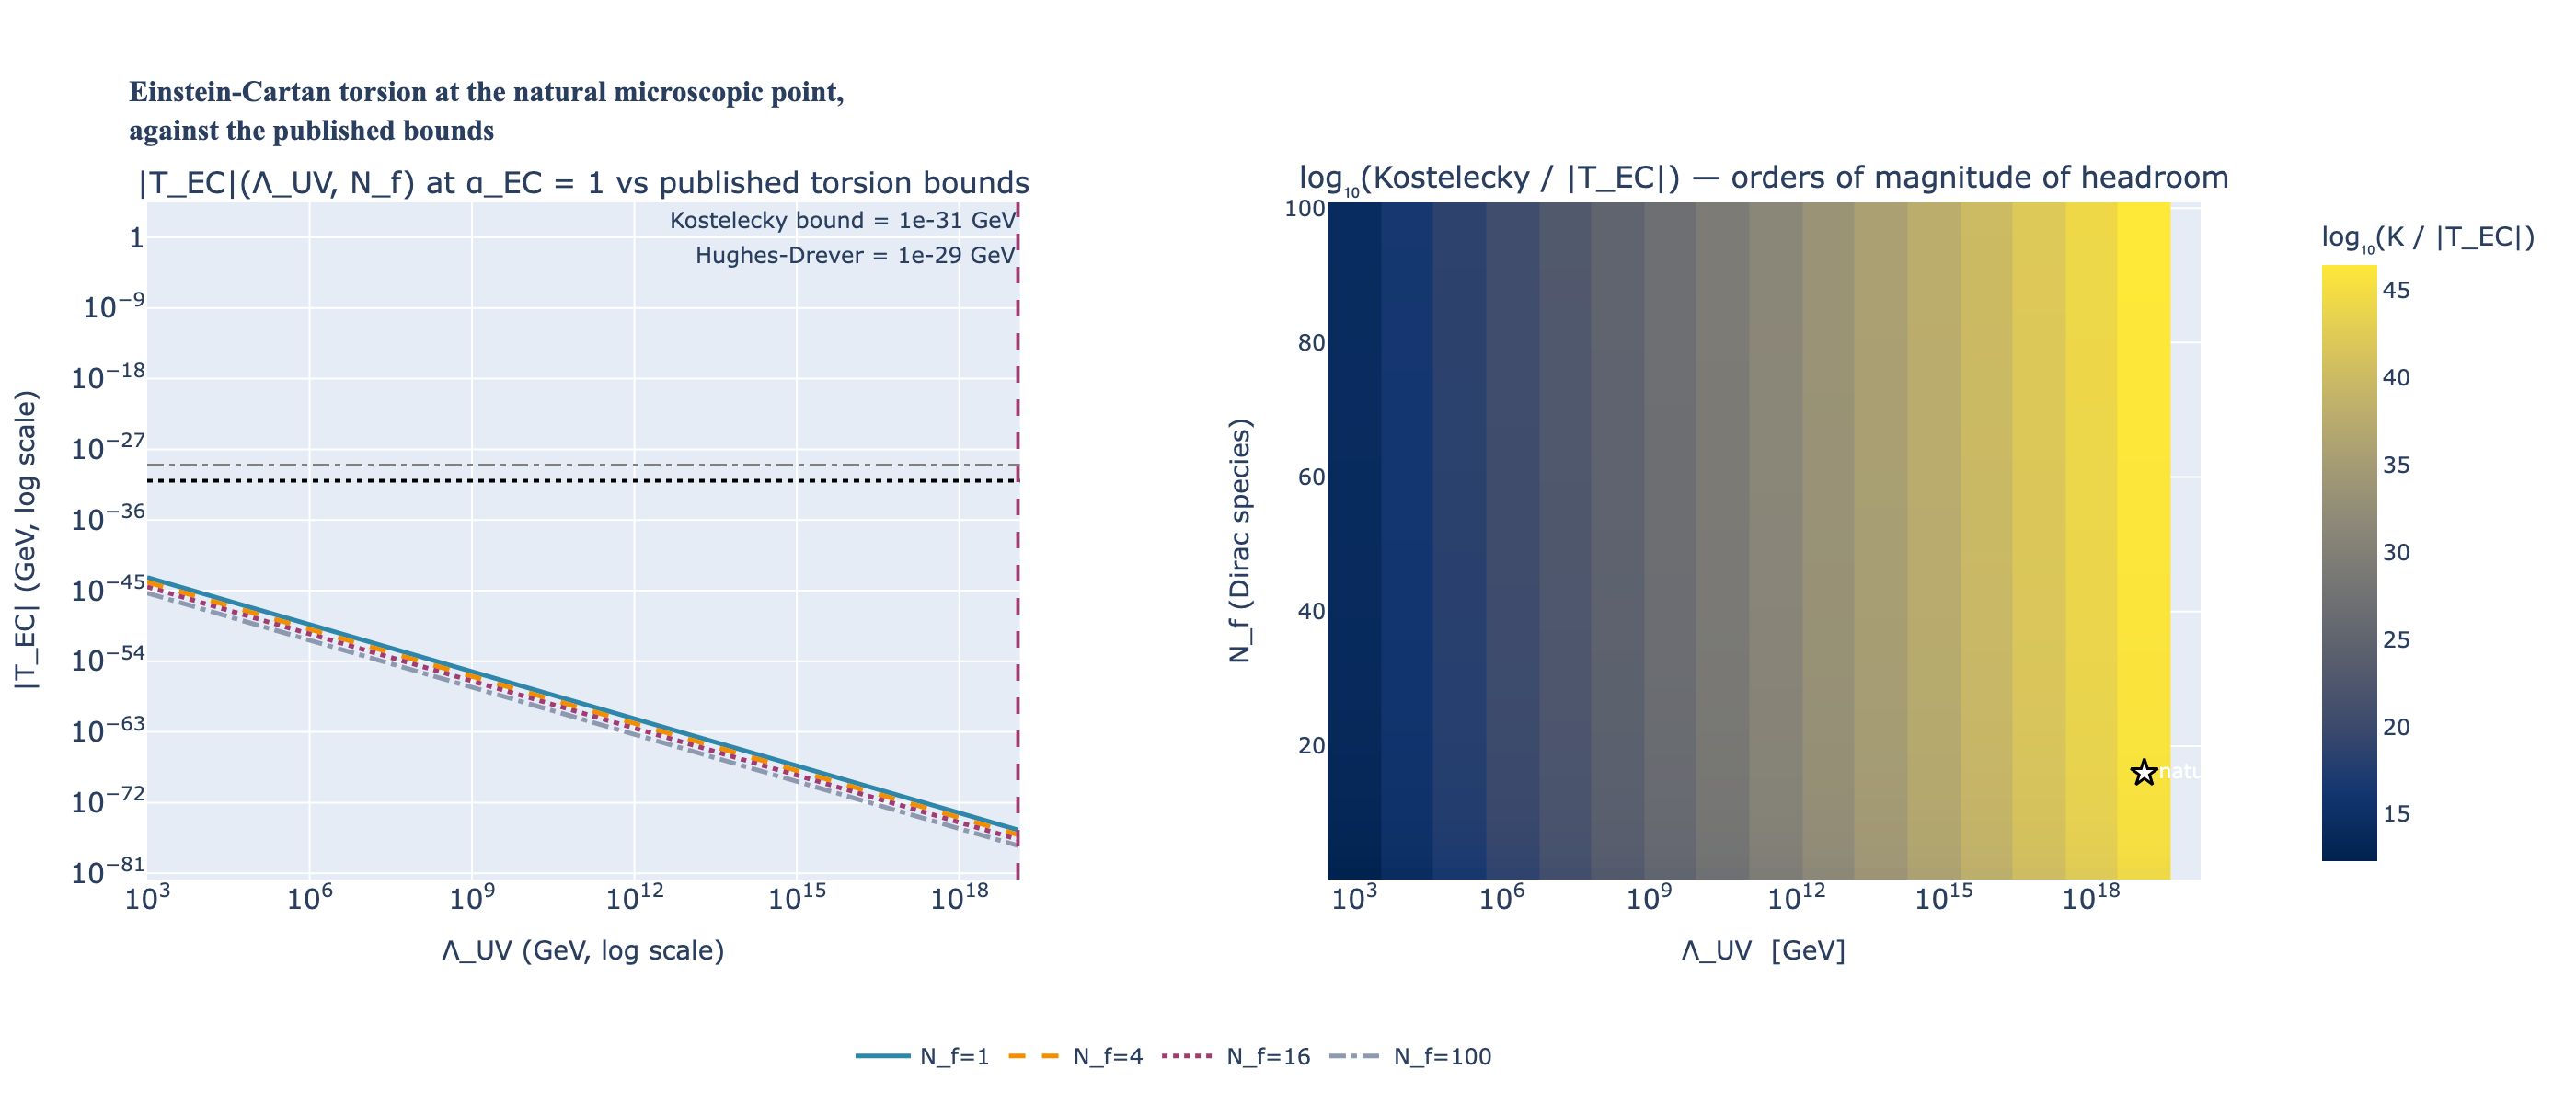
\includegraphics[width=\textwidth]{figures/fig_torsion_obs_bound.png}
\caption{The predicted torsion amplitude against the ceilings that constrain it.
Left: $|T_{\mathrm{EC}}|$ as a function of the cutoff $\Lambda_{\mathrm{UV}}$ at
$\alpha_{\mathrm{EC}} = 1$ for a range of species counts, with the tighter and
looser torsion ceilings drawn as horizontal lines and the Planck mass as a
vertical marker. Right: the base-ten logarithm of the ratio of the tighter
ceiling to the predicted amplitude across the $(\Lambda_{\mathrm{UV}}, N_f)$
plane. What the reader should take from the figure is that no point of the
parameter region approaches either ceiling. The margin is smallest at the
smallest cutoffs and at the smallest species counts, and it is still more than
ten orders of magnitude there, so the passage is a property of the construction
rather than of the operating point chosen.}
\label{fig:torsion-bound}
\end{figure*}

Unlike the quadratic-curvature comparison of \S\ref{sec:a4-two-ways}, the
torsion margin is not so large as to be uninformative about the future. The
amplitude scales as $\Lambda_{\mathrm{UV}}^{-2}$, so the prediction is a
falsifiable function of the cutoff rather than a number that would survive any
revision, and a torsion detection anywhere near the current sensitivity would
exclude the natural operating point outright.

%% =====================================================================
%% S8
%% =====================================================================
\section{What the formal substrate carries independently of the calibration}
\label{sec:bh-theorems}

Nothing in this section spends the heat-kernel coefficient. Every calibrated
statement so far has drawn on the same single piece of short-distance data, and a
reader arriving here after seven sections of that accounting is entitled to ask
where the budget has gone. It has not been touched. The singularity, area and
horizon-uniqueness content below is classical geometry formalised on its own
terms, and it stands whatever value the calibration takes. It earns its space
because it is the geometric ground on which the preceding thermodynamic
statements are read: an area law presupposes a horizon whose area is monotone, a
temperature is assigned to a horizon whose causal structure is fixed, and a
microscopic entropy is counted on a surface whose existence is a geometric
hypothesis. Machine-checking that layer, and stating exactly how far the machine
checking reaches, is what keeps the thermodynamic claims off an informal picture.

The scope caveat matters as much as the content, so we give it once and plainly.
What is formalised is a predicate layer. Causal relations, energy conditions,
null-expansion scalars and horizon areas are carried as propositions and as
real-valued functions of real parameters, and the theorems relate those
propositions to one another and discharge the real-analysis facts on which the
classical arguments turn. Curves, geodesics and affine completeness are not
modelled. No statement in this section is a machine-checked proof of a classical
singularity or uniqueness theorem, and at each point we say which part is a
derivation and which is a rearrangement of definitions.

\subsection{The singularity content and its exact reach}
\label{sec:bh-theorems-penrose}

The substrate declares a trapped surface directly on expansion data:
\texttt{Penrose\lb{}Singularity.\lb{}Is\lb{}Trapped\lb{}Surface} holds of a non-empty set of events
together with an outgoing and an ingoing null-expansion field when both
expansion scalars are strictly negative at every point of the set. The
singularity hypothesis \texttt{Penrose\lb{}Singularity.\lb{}Is\lb{}Penrose\lb{}Hypothesis\lb{}Satisfied}
is the conjunction of the null energy condition on a stress-energy bilinear form,
the trapped-surface predicate, and global hyperbolicity of the ambient causal
structure. The applicability predicate
\texttt{Penrose\lb{}Singularity.\lb{}Is\lb{}ADWPenrose\lb{}Applicable} is the purely geometric part
of that conjunction: trapped surface together with global hyperbolicity, with no
condition on the matter content.

The headline statement,
\texttt{Penrose\lb{}Singularity.\lb{}correctness\_\lb{}push\_\lb{}biconditional\_\lb{}under\_\lb{}applicable},
relates exactly these. Given the applicability predicate, the singularity
hypothesis holds if and only if the null energy condition holds for the
stress-energy form. Two things about this must be said in the open. First, the
right-hand side of the biconditional is the null energy condition and not
geodesic incompleteness; the theorem does not assert that anything is singular.
Second, because the applicability predicate is precisely the non-energy part of
the hypothesis, the equivalence is a projection of a conjunction onto its
remaining conjunct and a reconstruction of the conjunction from it. It is a
definitional unfolding relative to the applicability predicate, not a derivation.
Its worth is bookkeeping worth: it certifies that once the emergent geometry is
fixed, the energy condition on the emergent stress-energy is the single remaining
discriminator, so a later determination of that one predicate settles the
hypothesis outright.

The mathematical content of the focusing argument sits elsewhere, and it is a
genuine derivation. The substrate carries the closed-form Riccati solution
$\theta(\lambda) = \theta_0 / (1 + \theta_0 \lambda / 3)$ of
$\mathrm{d}\theta/\mathrm{d}\lambda = -\theta^2/3$ with $\theta(0) = \theta_0$,
which is the four-dimensional shear-free, curvature-suppressed form of the
focusing equation for the expansion of a null congruence. For $\theta_0 < 0$ the
denominator is strictly positive on $[0, -3/\theta_0)$, so the solution stays
strictly negative on that interval
(\texttt{Penrose\lb{}Singularity.\lb{}riccati\lb{}Solution\_\lb{}neg}), and the focal parameter
$-3/\theta_0$ is itself strictly positive
(\texttt{Penrose\lb{}Singularity.\lb{}focusing\lb{}Time\_\lb{}pos}). The statement that consumes the
full trapped-surface hypothesis rather than half of it is
\texttt{Penrose\lb{}Singularity.\lb{}penrose\_\lb{}both\_\lb{}focal\_\lb{}times\_\lb{}pos}: at any point of a
trapped surface, both the outgoing and the ingoing focal parameters are strictly
positive, so both null normal congruences focus at finite affine parameter. The
step from a finite focal parameter to failure of geodesic extension is the
curve-theoretic step, and it is not present. The conclusion predicate
\texttt{Penrose\lb{}Singularity.\lb{}Penrose\lb{}Conclusion} is defined, and the incompleteness
predicate it uses is carried as a positivity condition on an affine-parameter
bound rather than as a statement about a geodesic on a manifold; no theorem
derives that conclusion from the hypothesis. The classical statement associated
with Penrose~\cite{Penrose1965} is therefore not proved here, and we do not claim
it.

One non-degeneracy check is worth recording, because a predicate layer of this
kind can be made vacuous by accident. On the concrete one-dimensional causal
order used as the substrate's witness spacetime, a trapped surface cannot exist
once the expansion fields are non-negative
(\texttt{Penrose\lb{}Singularity.\lb{}real\lb{}Line\lb{}Spacetime\_\lb{}no\_\lb{}trapped\lb{}Surface\_\lb{}for\_\lb{}nonneg\_\lb{}expansion}),
so the trapped-surface predicate genuinely distinguishes the witness from a
four-dimensional geometry rather than holding everywhere.

\subsection{The strong-energy-condition variant is unavailable, and this follows
from the same number}
\label{sec:bh-theorems-hp}

The strong-energy variant associated with Hawking and
Penrose~\cite{HawkingPenrose1970} is formalised the same way, with the strong
energy condition replacing the null one:
\texttt{Hawking\lb{}Penrose\lb{}Singularity.\lb{}Is\lb{}Hawking\lb{}Penrose\lb{}Hypothesis\lb{}Satisfied} conjoins
the strong energy condition, the trapped-surface predicate and global
hyperbolicity, and
\texttt{Hawking\lb{}Penrose\lb{}Singularity.\lb{}hawking\lb{}Penrose\_\lb{}biconditional\_\lb{}under\_\lb{}applicable}
reduces it, under the same geometric applicability predicate, to the strong
energy condition alone. That reduction is the same definitional rearrangement as
above.

What is not a rearrangement is the obstruction. For a stress-energy form
$T_{\mu\nu} = -\Lambda g_{\mu\nu}$ on the flat metric, the strong-energy
combination evaluated on the explicit future-directed timelike witness
$v = (1,0,0,0)$, with the trace parameter carried as $-4\Lambda$, comes out equal
to $\Lambda\, g(v,v)$, which is strictly negative for every positive $\Lambda$.
That is \texttt{Energy\lb{}Conditions.\lb{}cosmological\lb{}Lambda\_\lb{}violates\_\lb{}SEC}, discharged
on an explicit witness rather than an existential. Feeding it into the hypothesis
gives \texttt{Hawking\lb{}Penrose\lb{}Singularity.\lb{}cosmological\lb{}Lambda\_\lb{}violates\_\lb{}HP\_\lb{}hypothesis}:
for every positive $\Lambda$, the strong-energy hypothesis fails outright on that
stress-energy.

This is where the section touches the spine of the paper. The emergent
cosmological constant of this framework is strictly positive, and that positivity
is itself machine-checked
(\texttt{Microscopic\lb{}Coefficient\lb{}Match.\lb{}lambda\lb{}Emerg\lb{}Microscopic\_\lb{}pos}). It is the same
constant whose magnitude is reported in \S\ref{sec:tests}, where its overshoot
against the observed value is the framework's sharpest quantitative liability.
Here the same number has a second consequence, and a purely structural one:
because the constant is positive, the substrate's own cosmological sector
violates the strong energy condition, and the strong-energy route to singularity
formation is therefore closed to it. Composing the two verified facts requires
nothing further, since the violation theorem is quantified over every positive
$\Lambda$.

We state the consequence as a result rather than as an omission. Singularity
formation in this framework has to be argued on the null energy condition alone,
by the route of \S\ref{sec:bh-theorems-penrose}; the stronger hypothesis is not
merely unproven here but unavailable in principle to a sector with a positive
cosmological constant. A referee weighing the cosmological-constant overshoot
should weigh this alongside it: one number carries both the quantitative cost and
this structural restriction, and both are consequences of the same positivity.

\subsection{The area theorem on the Schwarzschild family}
\label{sec:bh-theorems-area}

On the Schwarzschild family the horizon area is $A(M) = 16\pi M^2$, and its
monotonicity in the mass is discharged algebraically. For a mass history
$M : \mathbb{R} \to \mathbb{R}$ that is non-negative and non-decreasing, the
composed area history $t \mapsto A(M(t))$ is non-decreasing
(\texttt{Area\lb{}Theorem.\lb{}schwarzschild\_\lb{}horizon\_\lb{}area\_\lb{}non\lb{}Decreasing}), and on
strictly positive masses the dependence is strict: $0 < M_1 < M_2$ implies
$A(M_1) < A(M_2)$ (\texttt{Area\lb{}Theorem.\lb{}schwarzschild\_\lb{}area\_\lb{}strictly\_\lb{}increasing}).
The non-decreasing form is what the second law needs; the strict form is what
rules out an area that stalls under genuine accretion. Neither assumes anything
about the calibration, and both are elementary consequences of the closed form
together with monotonicity of squaring on the non-negative reals.

A second, curve-level statement carries the evolution content rather than the
closed form. Along a null generator parameterised by an affine parameter on a
compact interval, suppose the area obeys $A'(\lambda) = \theta(\lambda)
A(\lambda)$, is non-negative and continuous, and the expansion satisfies
$\theta(\lambda) \ge 0$ on the interior. Then the area is monotone
non-decreasing on the interval
(\texttt{Area\lb{}Theorem\lb{}Curve\lb{}Theoretic.\lb{}horizon\_\lb{}area\_\lb{}curve\_\lb{}monotone}). This is the
one-dimensional real-analysis core of the classical argument of
Hawking~\cite{Hawking1971}, and it is a derivation. The non-negativity of the
expansion is a hypothesis of the statement, encoding the reduction that the
classical argument performs from the null energy condition together with cosmic
censorship. That reduction is not itself formalised, so the theorem should be
read as: given non-negative expansion on the horizon generators, monotone area
follows rigorously.

The bridge to the thermodynamic reading is a positive rescaling. In units with
$G_N = 1$, a non-decreasing area function yields a non-decreasing
Bekenstein--Hawking entropy $S(t) = A(t)/4$
(\texttt{Area\lb{}Theorem.\lb{}area\_\lb{}theorem\_\lb{}implies\_\lb{}bh\_\lb{}entropy\_\lb{}monotone}). This gives
the geometric route to the second law of black-hole
mechanics~\cite{BardeenCarterHawking1973} independently of the dissipative
entropy-current argument and of the microscopic counting used earlier in this
paper, so the three routes converge on the same substrate without sharing an
input.

\subsection{The Kerr family and the sub-extremality bound}
\label{sec:bh-theorems-nohair}

The stationary family is carried as a parameter record
\texttt{No\lb{}Hair\lb{}Theorem.\lb{}Kerr\lb{}Family\lb{}Params} holding a mass $M$ and a signed angular
momentum $J$, with strict mass positivity and the sub-extremality condition
$J^2 \le M^4$ imposed as structural invariants rather than as later hypotheses.
Any inhabitant of that record therefore satisfies the bound by construction, and
the equivalent absolute-value form $|J| \le M^2$ is derived from it by a
square-root comparison (\texttt{No\lb{}Hair\lb{}Theorem.\lb{}subextremality\_\lb{}implies\_\lb{}abs\_\lb{}J\_\lb{}le\_\lb{}M\_\lb{}sq}).
This is where extremality enters the formal layer: parameters beyond the bound
are not merely undesirable, they cannot be constructed.

The $J = 0$ specialisation is discharged against the exact-solution machinery
rather than asserted. The zero-angular-momentum member has horizon radius
$r_+ = 2M$ (\texttt{No\lb{}Hair\lb{}Theorem.\lb{}kerr\_\lb{}family\_\lb{}schwarzschild\_\lb{}horizon\_\lb{}radius})
and horizon area $16\pi M^2$
(\texttt{No\lb{}Hair\lb{}Theorem.\lb{}kerr\_\lb{}family\_\lb{}schwarzschild\_\lb{}area}), matching the area used
in \S\ref{sec:bh-theorems-area}, and inherits the area monotonicity in the mass
(\texttt{No\lb{}Hair\lb{}Theorem.\lb{}kerr\_\lb{}family\_\lb{}schwarzschild\_\lb{}area\_\lb{}monotone}). These are
genuine cross-checks: they confirm that the parameterised family and the
independently defined Schwarzschild quantities agree where they overlap.

The statement named \texttt{No\lb{}Hair\lb{}Theorem.\lb{}no\lb{}Hair\lb{}Theorem\_\lb{}statement} requires care,
because its name promises more than its type delivers, and we would rather say so
than let a reader infer otherwise. Its antecedent predicate
\texttt{No\lb{}Hair\lb{}Theorem.\lb{}Is\lb{}Stationary\lb{}Axisymmetric\lb{}Vacuum\lb{}BH} is declared at this layer
without differential-geometric content: stationarity, axisymmetry, the vacuum
field equations and the presence of a horizon are named in its documentation but
are not modelled in its definition. Its conclusion,
\texttt{No\lb{}Hair\lb{}Theorem.\lb{}Has\lb{}Kerr\lb{}Family\lb{}Description}, asserts the existence of a
parameter record of positive mass and does not refer to the spacetime supplied to
it. The theorem, in consequence, fixes the interface between the two predicates
and constructs the witness through the $J = 0$ member; it establishes nothing
about uniqueness. Nothing in this paper should be read as a machine-checked proof
of black-hole uniqueness in the sense of Israel~\cite{Israel1967},
Carter~\cite{Carter1971}, Hawking~\cite{Hawking1972} or
Robinson~\cite{Robinson1975}.

Uniqueness content that is machine-checked exists, at a reduced scope, and is
worth separating from the above. The rigidity mechanism of the $\sigma$-model
argument distils to a real-analysis statement: a function that is continuous on a
compact interval, differentiable on its interior with non-negative derivative,
and takes equal values at the two endpoints is constant on the interval
(\texttt{Mazur\lb{}Sigma\lb{}Model\lb{}Rigidity.\lb{}mazur\_\lb{}monotone\_\lb{}rigidity}). Applying it to the
squared difference of a pair of Ernst potentials with matching boundary data
forces the two potentials to coincide throughout
(\texttt{Mazur\lb{}Sigma\lb{}Model\lb{}Rigidity.\lb{}ernst\_\lb{}potential\_\lb{}coincidence}). That is a
derivation, and it is the shape of the classical rigidity argument with the
elliptic and $\sigma$-model geometry replaced by its one-dimensional consequence;
the non-negativity of the derivative, which the classical argument obtains from
the divergence identity, is a hypothesis here. At the parameter level, two
records with equal mass and equal angular momentum are equal
(\texttt{Mazur\lb{}Sigma\lb{}Model\lb{}Rigidity.\lb{}kerr\lb{}Family\lb{}Params\_\lb{}unique\_\lb{}from\_\lb{}M\_\lb{}J}); this is
record extensionality over the two real fields, and it certifies that the
parameterisation carries no hidden data, not that the family is exhaustive.

\subsection{What this layer licenses}

Taken together, the results of this section license three readings and refuse a
fourth. They license the claim that the geometric hypotheses under which the
preceding thermodynamics is stated are written down precisely and are mutually
consistent, since the predicates are inhabited by an explicit witness and are not
satisfied vacuously. They license the focusing and monotonicity facts as
theorems, because those are real-analysis derivations with no gap. They license
the structural claim of \S\ref{sec:bh-theorems-hp}, which is a consequence of a
verified positivity and a verified counterexample. They do not license any claim
that the classical singularity, area or uniqueness theorems have been reproved by
machine; the curve-theoretic and elliptic steps that carry those theorems are
absent, and the predicate layer is honest scaffolding for them rather than a
substitute.

%% =====================================================================
%% S9
%% =====================================================================
\section{The strong-coupling voucher}
\label{sec:qcd}

The construction developed above was assembled for a dissipative hydrodynamic
layer and for the thermodynamics of the horizon it supports. This section
reports what that same construction says about the vacuum of quantum
chromodynamics, a sector it was not built to describe. Its placement at the
close of the paper is deliberate: nothing stated below fixed a coefficient, a
definition or a convention used earlier, so it is available as an independent
test rather than serving as a premise for anything that precedes it.

\subsection{Confinement as a statement about the centre}

A continuous gauge group leaves a discrete one-form symmetry exactly when it is
non-Abelian, which is how the substrate classifies gauge data
(\texttt{Center\lb{}Symmetry\lb{}Confinement.\lb{}higher\_\lb{}form\_\lb{}discrete\_\lb{}iff\_\lb{}non\_\lb{}abelian}).
For $\mathrm{SU}(N)$ that symmetry is the cyclic centre $\mathbb{Z}_N$,
generated by
\begin{equation}
\label{eq:centre-phase}
\zeta_N \;=\; \exp\!\big(2\pi i / N\big), \qquad N \ge 2 .
\end{equation}
The generator's algebraic content is discharged directly:
$\zeta_N^{\,N} = 1$
(\texttt{Center\lb{}Symmetry\lb{}Confinement.\lb{}center\lb{}Phase\_\lb{}pow\_\lb{}N}) and
$\lVert \zeta_N \rVert = 1$
(\texttt{Center\lb{}Symmetry\lb{}Confinement.\lb{}center\lb{}Phase\_\lb{}norm\_\lb{}one}), the second being
what makes the centre action a phase rotation and therefore invisible to the
loop's magnitude. The Polyakov loop~\cite{Polyakov1978} enters as a complex
value $P$, the centre acts by $P \mapsto \zeta_N P$, and the confining phase is
the locus $P = 0$.

That locus admits an order-parameter reading and a symmetry reading, and the
substrate carries each as a biconditional. The order-parameter reading,
$P$ confining if and only if $\lVert P \rVert = 0$
(\texttt{Center\lb{}Symmetry\lb{}Confinement.\lb{}confining\_\lb{}iff\_\lb{}magnitude\_\lb{}zero}), is
unconditional, and off the locus the magnitude is strictly positive
(\texttt{Center\lb{}Symmetry\lb{}Confinement.\lb{}deconfining\_\lb{}implies\_\lb{}magnitude\_\lb{}positive}).
The symmetry reading, $P$ confining if and only if $\zeta_N P = P$
(\texttt{Center\lb{}Symmetry\lb{}Confinement.\lb{}confining\_\lb{}iff\_\lb{}center\_\lb{}invariant}), carries
one hypothesis, $\zeta_N \neq 1$, without which invariance says nothing because
the centre element acts trivially.

The readings are content-equivalent because they share a left-hand side: they
compose into an equivalence between the number a lattice ensemble average
actually reports and the symmetry statement that gives the phase its meaning.
That exchange is made constantly and informally in the literature, and it is
worth having in a form where the exchange is licensed rather than assumed,
because it is not unconditional. Stating it formally forces the failure mode
into the open, as a hypothesis on $\zeta_N$ visible in the statement rather than
a side condition absorbed into a definition; the contrapositive half, that a
non-vanishing loop is not centre-invariant, consumes the same hypothesis
(\texttt{Center\lb{}Symmetry\lb{}Confinement.\lb{}nonzero\_\lb{}breaks\_\lb{}center\_\lb{}invariance}).

\subsection{Chiral symmetry breaking}

The Gell-Mann--Oakes--Renner relation~\cite{GellMannOakesRenner1968},
\begin{equation}
\label{eq:gmor}
m_\pi^2 f_\pi^2 \;=\; -2\, m_q \, \langle \bar q q \rangle ,
\end{equation}
ties the light pseudoscalar sector to the chiral condensate at first order in
the quark mass. The substrate discharges it numerically
(\texttt{Chiral\lb{}SSB\_\lb{}QCD.\lb{}gmor\_\lb{}pdg\_\lb{}match}): the left side is evaluated at
published central values for the pion mass and the pion decay constant, the
right side at a published central value for the mean light-quark mass and at a
lattice flavour average for the condensate, and the statement asserts that the
absolute difference falls below a tolerance fixed in $\mathrm{GeV}^4$ within the
theorem itself. The compilation of record for the measured meson and light-quark
properties is the Review of Particle Physics~\cite{PDG2024}. We are explicit
about the strength of the check: the tolerance is absolute rather than
fractional, and it is of the same order as the quantities being compared, so
what is certified is agreement at that scale and not agreement to a stated
number of significant figures.

The converse direction is sharper than the numerical match. A chiral-symmetric
vacuum, $\langle \bar q q \rangle \ge 0$, is inconsistent with
\eqref{eq:gmor} for any positive quark mass whenever the pion sector is
non-trivial: the left side is then strictly positive
(\texttt{Chiral\lb{}SSB\_\lb{}QCD.\lb{}gmor\_\lb{}lhs\_\lb{}pos\_\lb{}iff} gives positivity exactly when
$m_\pi$ and $f_\pi$ are both non-zero) while the right side is non-positive, and
the relation forces a contradiction
(\texttt{Chiral\lb{}SSB\_\lb{}QCD.\lb{}chiral\_\lb{}unbroken\_\lb{}violates\_\lb{}gmor}). This is a no-go on
the symmetric alternative, not a preference for the broken one.

Negativity of the condensate accordingly enters the substrate twice, and the
distinction matters. The type of condensates carries $\langle \bar q q\rangle <
0$ as an invariant of the type, which is what lets the positivity of the right
side of \eqref{eq:gmor} be read off for positive quark mass
(\texttt{Chiral\lb{}SSB\_\lb{}QCD.\lb{}gmor\_\lb{}rhs\_\lb{}pos\_\lb{}of\_\lb{}quark\_\lb{}mass\_\lb{}pos}). Taken alone that
would be an assumption wearing the costume of a result. The no-go is what
removes the circularity, because it is stated over an unconstrained real
condensate value and so cannot appeal to the invariant. A candidate value far
more negative than the observed one is rejected by the same machinery
(\texttt{Chiral\lb{}SSB\_\lb{}QCD.\lb{}not\_\lb{}is\lb{}Quark\lb{}Condensate\lb{}Candidate\_\lb{}of\_\lb{}too\_\lb{}negative}), so
the comparison predicate discriminates in both directions rather than accepting
anything negative.

\subsection{Colour-flavour locking}

At baryon densities high enough that the ordinary chiral condensate has
vanished, three-flavour quark matter condenses quark Cooper pairs in a channel
that breaks colour and flavour together, locking
$\mathrm{SU}(3)_{\mathrm{colour}} \times \mathrm{SU}(3)_L \times
\mathrm{SU}(3)_R$ to its diagonal subgroup and breaking chiral symmetry by a
mechanism unavailable at zero density, namely the locking of flavour rotations
to colour rotations~\cite[Eq.~(2.1) and \S2]{AlfordRajagopalWilczek1999}. The
substrate models the colour-flavour-locked phase by the diquark condensate's
value $\Phi$ and encodes the phase as a biconditional on its magnitude: the
system is colour-flavour locked if and only if $\lVert \Phi \rVert > 0$
(\texttt{CFLChiral\lb{}Lagrangian.\lb{}is\lb{}CFLPhase\_\lb{}iff\_\lb{}magnitude\_\lb{}pos}), the same shape
of statement as the Polyakov-loop order parameter above and deliberately so.
The accompanying Lagrangian skeleton carries a mass term proportional to
$m_q \lVert \Phi \rVert^2$, vanishing in the chiral limit
(\texttt{CFLChiral\lb{}Lagrangian.\lb{}cfl\lb{}Mass\lb{}Term\_\lb{}chiral\_\lb{}limit}) and strictly positive
in the locked phase at positive quark mass
(\texttt{CFLChiral\lb{}Lagrangian.\lb{}cfl\lb{}Mass\lb{}Term\_\lb{}pos\_\lb{}in\_\lb{}cfl\_\lb{}phase}).

The result this subsection exists for concerns the cube root of unity that
governs the dense phase. In the substrate the diquark sector's generator is
written $\omega = \exp(2\pi i/3)$ and the gauge centre's generator is
$\zeta_3$ of \eqref{eq:centre-phase}, and
\texttt{CFLChiral\lb{}Lagrangian.\lb{}CFL\_\lb{}emergent\_\lb{}Z3\_\lb{}matches\_\lb{}QCD\_\lb{}center\_\lb{}Z3} states
$\omega = \zeta_3$. What that establishes should be stated precisely. The
symbols are introduced in separate modules, but they are the same closed form,
and the equality holds by unfolding the definitions; it records an
identification rather than deriving one, and it is not evidence that an emergent
symmetry of the dense phase must coincide with the gauge centre of the vacuum
theory. What it does secure is transport. The algebraic facts on the diquark
side are proved through the identification rather than reproved from scratch, so
$\omega^3 = 1$ (\texttt{CFLChiral\lb{}Lagrangian.\lb{}emergent\lb{}Z3\_\lb{}pow\_\lb{}3}) and
$\lVert \omega \rVert = 1$
(\texttt{CFLChiral\lb{}Lagrangian.\lb{}emergent\lb{}Z3\_\lb{}norm\_\lb{}one}) are literally the
centre-side facts and cannot drift from them as the development grows, and the
cube roots of unity sum to zero
(\texttt{CFLChiral\lb{}Lagrangian.\lb{}emergent\lb{}Z3\_\lb{}sum\_\lb{}cube\_\lb{}roots}), which is the
algebraic content that distinguishes $\mathbb{Z}_3$ from the $\mathbb{Z}_2$ case.

The physical warrant for making that identification is external to the
substrate, and it is narrower than the identification. In the
colour-flavour-locked phase the braiding of a colour Wilson loop with a vortex
worldsheet carries a phase equal to a cube root of unity, and the symmetry this
generates is an emergent $\mathbb{Z}_3$ \emph{two-form} symmetry whose charged
objects are the vortices~\cite[Eqs.~(24)--(25)]{HironoTanizaki2018}. That
analysis concludes that the emergent symmetry cannot be spontaneously broken,
since the vortex interaction is logarithmically confining, so the phase carries
no deconfined topological excitation and quark-hadron continuity survives as a
scenario. What recurs across the sectors, then, is the cube root itself, and the
substrate's identification is faithful to that much and no more.

The chiral and dense sectors are also coupled inside the substrate. A
colour-flavour-locked configuration together with \eqref{eq:gmor} at positive
quark mass forces the condensate to be negative and the diquark magnitude to be
strictly positive at once
(\texttt{CFLChiral\lb{}Lagrangian.\lb{}cfl\_\lb{}phase\_\lb{}with\_\lb{}gmor\_\lb{}dual\_\lb{}broken}), so the
symmetry breaking in the light sector and the condensation in the dense sector
are not independent bookkeeping.

\subsection{What agreement of this kind constrains}

The statements above are facts about strongly coupled gauge dynamics: a
confinement criterion, a soft-pion relation between the pion sector and the
chiral condensate, and the discrete symmetry of a dense colour-superconducting
phase. None of them was a design target of the construction, and none of them is
accessible to the weak-coupling expansions the earlier sections use. They reach
the substrate through one channel only, the discrete data left behind when a
continuous non-Abelian gauge symmetry is reduced: the centre $\mathbb{Z}_N$, its
generator, and the finite fusion data attached to it, whose simple objects are
counted by the order of the centre
(\texttt{Center\lb{}Symmetry\lb{}Confinement.\lb{}su3k1\_\lb{}fusion\_\lb{}card\_\lb{}matches\_\lb{}z3\_\lb{}order}).

That is the same classification the horizon construction of
\S\ref{sec:entropy} consumes. The categories involved are not the same object,
and we do not claim they are: the horizon carries its own modular category while
the strong-coupling statements here concern the $\mathrm{SU}(3)_1$ data. What is
shared is the classifier and the arithmetic of the centre, and a substrate whose
higher-form data were wrong in that respect would fail on both sides at once.
Agreement therefore does not confirm the horizon results, and we do not offer it
as confirmation. It removes a way those results could have been wrong, in a
regime where an error would have had nowhere to hide, and it does so on facts
that were fixed by measurement long before any of this machinery existed.

%% =====================================================================
%% S10
%% =====================================================================
\section{Scope}
\label{sec:scope}

This section states what the preceding claims cover, what they exclude, and what
would overturn them. It is placed at the end because several of its entries can
only be read against the results they qualify.

\subsection{What the coefficient closed}
\label{sec:scope-closures}

Routes to a classical metric that this construction eliminates are collected
here once, rather than left distributed across the sections that derive them,
because they share a mechanism: each is decided by numbers the calibration of
\S\ref{sec:substrate} produces, and none of them requires an additional input.
A perturbative string-net route induces a four-fermion coupling whose ratio to
the condensation threshold is $\alpha^2 N_f/(32\pi^3)$, in which the cutoff
cancels, so there is no ultraviolet scale at which the perturbative route
reaches the threshold. Coarse-graining to a hydrodynamic layer keeps a gauge
sector exactly when its group is Abelian, so the colour and weak sectors carry
no hydrodynamic mode and cannot constrain the substrate's coarse-grained
description; the gravitational sector is where the coefficient is testable and
the only place it is. The substrate's own vestigial phase, which carries a
metric bilinear without a tetrad, propagates a spin-two disturbance at
$c\sqrt{\chi_{\mathrm{vest}}}$, and the multi-messenger timing of GW170817
admits it only on an interval of $\chi_{\mathrm{vest}}$ interior to the natural
range and narrower by more than fourteen orders of magnitude. That last result
is a constraint and not an exclusion, and it should not be read as one: the
phase survives, at the price of a susceptibility pinned to unity by something
the construction does not supply. Order-$a_4$ invariance, in the algebraic sense
of \S\ref{sec:tests}, admits the Dirac coefficient assignment and no deformation
of it, with the obstruction available in closed form rather than as a
non-existence claim.

\subsection{What the negative results are}
\label{sec:scope-negatives}

Two results are unfavourable to the construction and are reported as results
rather than as exceptions to a clearance list.

The emergent cosmological constant overshoots the observed value by more than a
hundred orders of magnitude at the fiducial point, and the overshoot arises from
the leading heat-kernel coefficient, which is fixed by the same species count
that fixes $G_N$ and is therefore not adjustable. Nothing in the construction
supplies a counterterm or a symmetry that would cancel it, and the emergent
value is positive. This answers, in the negative, the standing question of
whether obtaining the gravitational coupling from matter loops relieves the
vacuum-energy problem, and it answers it inside the computation that produced
$G_N$ rather than in a separate sector where the answer could be attributed to
an unrelated approximation.

The strong-energy-condition route to singularity formation is unavailable to
this substrate, and for the same reason. A positive cosmological constant
violates the strong energy condition on an explicit timelike witness, so the
singularity theorem that requires it does not apply here and singularity
formation has to be argued on the null condition alone. One number carries the
quantitative liability and this structural restriction together.

\subsection{What is formalised, and what the formalisation does not reach}
\label{sec:scope-formal}

The machine-checked layer is cited by theorem name throughout, and the reach of
each statement is given where its name promises more than its type delivers. The
recurring pattern is worth stating once. Algebraic and real-analytic content is
formalised in full: the gap equation and its threshold, the heat-kernel
coefficient identities, the trace-level field equations and the post-Newtonian
channel relations, the propagation-speed inequality and the interval it leaves,
the Stirling-with-remainder asymptotics behind the entropy's subleading
logarithm, the classification biconditional at the regime-partition mass, the
torsion comparison, and the curvature-density identities of the
quadratic-curvature sector. Differential-geometric content is not. There are no
curves, no geodesics and no affine completeness in the formal layer, so no
statement in \S\ref{sec:bh-theorems} is a machine-checked proof of a classical
singularity, area or uniqueness theorem, and the statement carrying the
no-hair name asserts the existence of a parameter record rather than the
uniqueness of a solution. Tensorial field equations on a manifold are likewise
outside the layer, which works with the linearised sector, the trace, and the
cosmological reduction. Where a classical argument is reduced to its
one-dimensional analytic core, the reduction step is a hypothesis of the
formalised statement and is named as one: the non-negativity of the horizon
generators' expansion in the area theorem, the non-negativity of the derivative
in the rigidity argument, and the evaporation-sign fields of the regime
partition are all transported rather than derived.

Two further scope statements belong here because they cross sections. The
substrate-class record of \S\ref{sec:regime} is a classification recorded on
hand-declared data, verified in the sense that the record has been read
correctly and not in the sense that the physics behind an entry has been
derived, and the bridge from it to a horizon fluctuation theorem is stated as a
target rather than proved. And the identification in \S\ref{sec:qcd} of the
colour-flavour-locked cube root with the generator of the gauge centre holds by
unfolding the definitions; what it secures is that the algebraic facts on the
two sides cannot drift apart, not that an emergent symmetry of the dense phase
has been derived to coincide with the vacuum theory's centre.

\subsection{What would falsify the construction}
\label{sec:scope-falsifiers}

The construction is exposed in several independent places, and it is worth
separating the exposures that current sensitivity can reach from those it
cannot.

Within reach now: the post-Newtonian channels of \S\ref{sec:efe} form a
one-parameter family, so the perihelion deviation must be two-thirds of the
deflection deviation with $\alpha_{\mathrm{ADW}}$ already eliminated between
them; a measurement of the two in any other proportion falsifies the
construction without determining $\alpha_{\mathrm{ADW}}$ at all. The torsion
amplitude of \S\ref{sec:tests} scales as $\Lambda_{\mathrm{UV}}^{-2}$, so a
detection of background torsion anywhere near current Lorentz-violation
sensitivity excludes the fiducial point outright. A gravitational-wave
propagation speed differing from the electromagnetic one by more than the
GW170817 cap, in any future event, closes the vestigial branch entirely rather
than merely confining it.

Within reach of theory rather than measurement: the horizon entropy's
logarithmic coefficient is derived from the state count of a non-abelian
category, and a macroscopic computation of the same coefficient for the same
black hole disagrees with it in sign. That disagreement is unresolved here and
is stated because it is the sharpest available test of the horizon category. An
abelian horizon category fails the boundary condition before the subleading term
is reached, so a demonstration that the substrate's horizon must carry abelian
fusion data would remove the entropy account entirely.

Not currently a test: the quadratic-curvature couplings clear the ceiling they
are compared against by many tens of orders of magnitude, and any construction
whose quadratic couplings come from a one-loop determinant would clear it
equally. Passing there is the absence of an exclusion and is not evidence.

\subsection{What the paper does not claim}
\label{sec:scope-nonclaims}

It does not claim that $\alpha_{\mathrm{ADW}} = 1$ has been derived. It does not
claim that the classical singularity, area or uniqueness theorems have been
reproved by machine. It does not claim that the observed Newton constant is
predicted; what is predicted is the relation among channels once the constant is
matched, and the matching places the cutoff at an order-unity multiple of the
Planck mass rather than at a tuned value. It does not claim that the
cosmological-constant problem is solved, or softened, or made more tractable by
being emergent. And it does not claim that the agreement of \S\ref{sec:qcd}
confirms the gravitational results, because the categories involved are not the
same object; what that agreement removes is a way the higher-form data could
have been wrong, in a regime where an error would have had nowhere to hide.

%% =====================================================================
%% Appendix
%% =====================================================================
\appendix

\section{The algebraic Lorentzian-geometry substrate}
\label{app:lorentzian-substrate}

This appendix records the geometric layer that
\S\ref{sec:bh-theorems} consumes. It is written to be consulted rather than read
through, and it is needed because general-purpose formalised-mathematics
libraries currently supply Riemannian, that is positive-definite, metric
structure, together with a covariant-derivative and torsion interface, but no
indefinite-signature counterpart, no curvature objects built on that interface,
and no causal structure. Each item below states what is defined, what is proved,
and where the boundary of the proof lies.

\paragraph{Indefinite-signature metric structure.}
At the matrix level, \texttt{Lorentzian\lb{}Metric.\lb{}Is\lb{}Lorentzian\lb{}Signature} asserts of a
$4 \times 4$ real array that the time-time entry is $-1$, the remaining diagonal
entries are $+1$, and the off-diagonal entries vanish;
\texttt{Lorentzian\lb{}Metric.\lb{}Is\lb{}Lorentzian\lb{}Metric} adds symmetry and non-degeneracy, and
the Minkowski array is verified to satisfy it. The separation from the
positive-definite case is proved rather than asserted: a positive-definite form
cannot satisfy the Lorentzian signature predicate
(\texttt{Lorentzian\lb{}Metric.\lb{}riemannian\_\lb{}not\_\lb{}lorentzian\_\lb{}signature}). At the bundle
level, \texttt{Lorentzian\lb{}Bundle.\lb{}Is\lb{}Lorentzian\lb{}Bundle} asks of a family of fibrewise
bilinear forms on the tangent spaces only that each be symmetric and
non-degenerate. Positive-definiteness is nowhere assumed, which is the point:
the constructions below are semi-Riemannian and apply to indefinite signature
without modification. Non-degeneracy yields injectivity of the pairing in either
slot (\texttt{Lorentzian\lb{}Bundle.\lb{}lorentzian\lb{}Bundle\_\lb{}pairing\_\lb{}left\_\lb{}injective} and
\texttt{Lorentzian\lb{}Bundle.\lb{}lorentzian\lb{}Bundle\_\lb{}pairing\_\lb{}right\_\lb{}injective}).

\paragraph{Levi-Civita uniqueness by the Koszul formula.}
At the matrix level the Koszul closed form for the Christoffel symbols is
defined with the metric partial derivatives supplied as explicit inputs rather
than computed, which makes the resulting identities independent of any coordinate
apparatus, and it is proved symmetric in its lower indices
(\texttt{Riemannian\lb{}Connection.\lb{}christoffel\lb{}Koszul\_\lb{}is\lb{}Torsion\lb{}Free}). At the bundle
level the substantive uniqueness argument is carried in full. The predicate
\texttt{Levi\lb{}Civita.\lb{}Is\lb{}Levi\lb{}Civita} conjoins the covariant-derivative interface,
torsion-freeness, symmetry of the fibre metric, and metric compatibility
expressed through the exterior derivative of the scalar pairing. From it the
Koszul identity is derived
(\texttt{Levi\lb{}Civita.\lb{}koszul\_\lb{}identity\_\lb{}of\_\lb{}is\lb{}Levi\lb{}Civita}), and two connections
satisfying the predicate for the same metric are shown to agree pointwise
(\texttt{Levi\lb{}Civita.\lb{}levi\lb{}Civita\_\lb{}unique\_\lb{}of\_\lb{}is\lb{}Levi\lb{}Civita}). The specialisation to
the indefinite-signature case is
\texttt{Lorentzian\lb{}Bundle.\lb{}levi\lb{}Civita\_\lb{}unique\_\lb{}for\_\lb{}lorentzian\lb{}Bundle}, which supplies
the non-degeneracy input from the symmetric non-degenerate fibre metric directly.

\paragraph{The algebraic first Bianchi identity.}
For a covariant derivative on the tangent bundle that is torsion-free in the
sense that the antisymmetrised derivative of two sections equals their Lie
bracket, the cyclic sum of the curvature operator vanishes:
$R(X,Y)Z + R(Y,Z)X + R(Z,X)Y = 0$
(\texttt{Bundle\lb{}Riemann.\lb{}bundle\lb{}Riemann\lb{}Aux\_\lb{}first\_\lb{}bianchi\_\lb{}torsionfree\_\lb{}apply}, with
the variant \texttt{bundle\lb{}Riemann\lb{}Aux\_\lb{}first\_\lb{}bianchi\_\lb{}torsionfree\_\lb{}of\_\lb{}is\lb{}Covariant\lb{}Derivative\lb{}On}
that consumes the library's covariant-derivative interface in place of an
abstract additivity hypothesis). The proof runs through a pointwise cyclic Jacobi
identity for the manifold Lie bracket
(\texttt{Bundle\lb{}Riemann.\lb{}mlie\lb{}Bracket\_\lb{}cyclic\_\lb{}jacobi\_\lb{}apply}), which is derived from
the library's Leibniz form together with antisymmetry and pointwise negation
distribution. Two scope points: no metric enters this statement, so it is
signature-agnostic and holds for indefinite signature as a special case; and the
identity is the algebraic one, the differential second Bianchi identity being
supported only through antisymmetry machinery elsewhere.

\paragraph{Algebraic Riemann and Einstein tensors.}
The Christoffel-quadratic part of the Riemann tensor is defined and proved
antisymmetric in its last index pair
(\texttt{Riemannian\lb{}Connection.\lb{}riemann\lb{}Quadratic\lb{}Term\_\lb{}Antisym\lb{}Last\lb{}Two}); the part
involving derivatives of the Christoffel symbols is outside this scope. The
Einstein tensor is defined as $G_{\mu\nu} = R_{\mu\nu} - \tfrac{1}{2} R
g_{\mu\nu}$, is symmetric when the Ricci tensor and the metric are
(\texttt{Einstein\lb{}Tensor.\lb{}einstein\lb{}Tensor\_\lb{}symm}), and satisfies the
dimension-dependent trace identity $G^{\mu}{}_{\mu} = -R$, where the dimension
enters through the contraction of the metric with its inverse
(\texttt{Einstein\lb{}Tensor.\lb{}einstein\lb{}Tensor\_\lb{}trace\_\lb{}eq\_\lb{}neg\_\lb{}scalar}). The vacuum
characterisation $G_{\mu\nu} = 0 \Leftrightarrow R_{\mu\nu} = 0$ is a
biconditional with the dimension contraction as a load-bearing hypothesis
(\texttt{Einstein\lb{}Tensor.\lb{}einstein\lb{}Tensor\_\lb{}zero\_\lb{}iff\_\lb{}ricci\_\lb{}zero}), and for the
constant-sectional-curvature witness the $\Lambda$-vacuum equation is equivalent
to $\Lambda = 3K$ (\texttt{Einstein\lb{}Tensor.\lb{}constant\lb{}Sectional\_\lb{}lambda\_\lb{}vacuum\_\lb{}iff}).

\paragraph{Energy conditions.}
The null, weak, dominant and strong energy conditions are predicates on an
abstract stress-energy bilinear form paired with a metric, in signature
$(-,+,+,+)$, with the timelike and null restrictions load-bearing in each case
and the trace supplied externally for the strong condition. The chain from
dominant to weak is a projection
(\texttt{Energy\lb{}Conditions.\lb{}DEC\_\lb{}implies\_\lb{}WEC}); the step from weak to null carries
its approximation hypothesis explicitly, as a sequence of future-directed
timelike vectors along which the stress-energy converges
(\texttt{Energy\lb{}Conditions.\lb{}WEC\_\lb{}implies\_\lb{}NEC\_\lb{}under\_\lb{}continuity}). Non-implications
are witnessed by explicit tensors and explicit vectors rather than by
existentials: the cosmological-constant form satisfies the weak and null
conditions and violates the strong one
(\texttt{Energy\lb{}Conditions.\lb{}cosmological\lb{}Lambda\_\lb{}WEC},
\texttt{Energy\lb{}Conditions.\lb{}cosmological\lb{}Lambda\_\lb{}NEC},
\texttt{Energy\lb{}Conditions.\lb{}cosmological\lb{}Lambda\_\lb{}violates\_\lb{}SEC}); a ghost scalar with
spacelike gradient violates the null condition
(\texttt{Energy\lb{}Conditions.\lb{}ghost\lb{}Scalar\_\lb{}violates\_\lb{}NEC}); and a perfect fluid with
pressure exceeding density violates the dominant condition on a named pair of
future-directed timelike vectors
(\texttt{Energy\lb{}Conditions.\lb{}stiff\_\lb{}fluid\_\lb{}violates\_\lb{}DEC}).

\paragraph{Tetrad and metric.}
The tetrad-induced metric $g_{\mu\nu} = \eta_{ab} e^a{}_\mu e^b{}_\nu$ is defined
by explicit contraction and proved symmetric for every tetrad configuration
(\texttt{Tetrad\lb{}Formalism.\lb{}tetrad\lb{}Induced\lb{}Metric\_\lb{}symm}), and the canonical frame
$e^a{}_\mu = \delta^a{}_\mu$ recovers the flat metric exactly
(\texttt{Tetrad\lb{}Formalism.\lb{}minkowski\lb{}Tetrad\_\lb{}induces\_\lb{}minkowski\_\lb{}metric}). The
reduction of the tetrad formulation to the metric formulation is tied to the
vanishing of the torsion residual, which happens exactly at unit Einstein--Cartan
parameter (\texttt{Tetrad\lb{}Formalism.\lb{}tetrad\_\lb{}levi\_\lb{}civita\_\lb{}iff\_\lb{}alpha\_\lb{}unity}). The
converse direction, recovery of a tetrad from a metric up to local Lorentz
transformation, is not formalised.

\paragraph{Canonical constraints.}
The Hamiltonian and momentum constraints of the canonical
formulation~\cite{ADM1962} are carried as scalar relations among the spatial
scalar curvature, the trace and squared norm of the extrinsic curvature, and the
matter density and current. In vacuum the Hamiltonian constraint is equivalent to
$^{(3)}R + (\mathrm{tr}\,K)^2 = K_{ij}K^{ij}$
(\texttt{ADMFormalism.\lb{}hamiltonian\lb{}Constraint\_\lb{}vacuum\_\lb{}iff}), at a moment of time
symmetry it reduces to $^{(3)}R = 16\pi\rho$
(\texttt{ADMFormalism.\lb{}hamiltonian\lb{}Constraint\_\lb{}moment\_\lb{}of\_\lb{}time\_\lb{}symmetry\_\lb{}iff}), and
in vacuum the momentum constraint is equivalent to vanishing of the trace-free
divergence (\texttt{ADMFormalism.\lb{}momentum\lb{}Constraint\_\lb{}vacuum\_\lb{}iff}). The spatial
covariant divergence is an input to these statements rather than a computed
quantity, so the constraints are verified as scalar identities in the curvature
invariants and not at tensorial scope. Flat space satisfies both
(\texttt{ADMFormalism.\lb{}minkowski\_\lb{}satisfies\_\lb{}hamiltonian\lb{}Constraint},
\texttt{ADMFormalism.\lb{}minkowski\_\lb{}satisfies\_\lb{}momentum\lb{}Constraint}).

\paragraph{Causal structure and its witness.}
A spacetime is carried as a topological space of events with a causal and a
chronological relation subject to reflexivity of the causal relation,
transitivity of both, containment of the chronological relation in the causal
one, and mixed transitivity in either order. Causal and chronological futures and
pasts are the set-valued projections of these relations. The hierarchy is
declared as predicates: absence of closed timelike loops; antisymmetry of the
causal relation; causal convexity of small neighbourhoods; existence of a
continuous time function strictly increasing along chronological pairs; and
global hyperbolicity, defined as causal convexity together with compactness of
every causal diamond. Only one downward implication is proved, and it is proved
honestly: a strictly monotone continuous time function rules out closed timelike
loops
(\texttt{Causal\lb{}Structure.\lb{}Spacetime.\lb{}Is\lb{}Stably\lb{}Causal\_\lb{}implies\_\lb{}Is\lb{}Chronological}). The
implication from causal antisymmetry to absence of closed timelike loops is
recorded as not derivable from the relational axioms alone, because the textbook
argument uses a notion of curve length that the relational layer cannot express,
and it is deliberately not shipped. The witness is the real line ordered by
$\le$ and $<$, which is verified to have no closed timelike loops
(\texttt{Causal\lb{}Structure.\lb{}Spacetime.\lb{}real\lb{}Line\lb{}Spacetime\_\lb{}is\lb{}Chronological}), to be
causally antisymmetric
(\texttt{Causal\lb{}Structure.\lb{}Spacetime.\lb{}real\lb{}Line\lb{}Spacetime\_\lb{}is\lb{}Causal}), to admit the
identity as a time function
(\texttt{Causal\lb{}Structure.\lb{}Spacetime.\lb{}real\lb{}Line\lb{}Spacetime\_\lb{}is\lb{}Stably\lb{}Causal}), to have
causal and chronological futures equal to the closed and open upper half-lines,
and to have causal diamonds equal to closed bounded intervals
(\texttt{Causal\lb{}Structure.\lb{}Spacetime.\lb{}real\lb{}Line\lb{}Spacetime\_\lb{}causal\lb{}Diamond\_\lb{}eq}), which
supplies the compactness input to global hyperbolicity by Heine--Borel. Every
singleton is a Cauchy surface for it
(\texttt{Causal\lb{}Structure.\lb{}Spacetime.\lb{}real\lb{}Line\lb{}Spacetime\_\lb{}singleton\_\lb{}is\lb{}Cauchy\lb{}Surface}).

\paragraph{Candidates for a general-purpose library.}
Several items above are stated at library generality rather than at the
generality this paper needs, and are natural candidates for contribution to a
general-purpose formalised-mathematics library such as Mathlib4. The
symmetric non-degenerate fibre-metric predicate and its pairing-injectivity
consequences are signature-agnostic and phrased over an arbitrary nontrivially
normed field. The pointwise cyclic Jacobi identity for the manifold Lie bracket
and the pointwise negation-distribution lemmas it rests on fill an identified gap
beside the library's existing Leibniz form. The algebraic first Bianchi identity
for torsion-free covariant derivatives on the tangent bundle, and the
Koszul-formula derivation and Levi-Civita uniqueness theorem for any
non-degenerate symmetric fibre metric, are stated over the same generality and
depend on the library's covariant-derivative interface rather than on anything
specific to this paper. The predicate layers that are specialised to four
dimensions or to a fixed index set, in particular the matrix-level signature
predicates, the energy conditions and the canonical constraints, are not offered
in that form.

\begin{thebibliography}{99}

\bibitem{Abbott2017GW170817}
B.~P.~Abbott \emph{et al.} (LIGO+Virgo+EM partners),
``Gravitational waves and gamma-rays from a binary neutron star merger:
GW170817 and GRB 170817A,''
Astrophys.\ J.\ Lett.\ \textbf{848}, L13 (2017),
arXiv:1710.05834.

\bibitem{Adler1980}
S.~L.~Adler,
``Order-$R$ vacuum action functional in scalar-free unified theories
with spontaneous scale breaking,''
Phys.\ Rev.\ Lett.\ \textbf{44}, 1567 (1980).

\bibitem{ADM1962}
R.~Arnowitt, S.~Deser, and C.~W.~Misner,
``The dynamics of general relativity,''
Gen.\ Rel.\ Grav.\ \textbf{40}, 1997 (2008),
arXiv:gr-qc/0405109. Originally Chapter 7 in
\emph{Gravitation: An Introduction to Current Research}, ed.\ Witten
(Wiley, 1962).

\bibitem{Akama1978}
K.~Akama,
``An attempt at pregeometry: gravity with composite metric,''
Prog.\ Theor.\ Phys.\ \textbf{60}, 1900 (1978).

\bibitem{AlfordRajagopalWilczek1999}
M.~G.~Alford, K.~Rajagopal, and F.~Wilczek,
``Color-flavor locking and chiral symmetry breaking in high density QCD,''
Nucl.\ Phys.\ B \textbf{537}, 443 (1999),
arXiv:hep-ph/9804403.

\bibitem{Balbinot2005PRD}
R.~Balbinot, S.~Fagnocchi, and A.~Fabbri,
``Quantum effects in acoustic black holes: the backreaction,''
Phys.\ Rev.\ D \textbf{71}, 064019 (2005),
arXiv:gr-qc/0405098.

\bibitem{BardeenCarterHawking1973}
J.~M.~Bardeen, B.~Carter, and S.~W.~Hawking,
``The four laws of black hole mechanics,''
Commun.\ Math.\ Phys.\ \textbf{31}, 161 (1973).

\bibitem{Carter1971}
B.~Carter,
``Axisymmetric black hole has only two degrees of freedom,''
Phys.\ Rev.\ Lett.\ \textbf{26}, 331 (1971).

\bibitem{Diakonov2011}
D.~Diakonov,
``Towards lattice-regularized quantum gravity,''
arXiv:1109.0091 (2011).

\bibitem{Eddington1919}
F.~W.~Dyson, A.~S.~Eddington, and C.~Davidson,
``A determination of the deflection of light by the Sun's gravitational
field, from observations made at the total eclipse of May 29, 1919,''
Philos.\ Trans.\ R.\ Soc.\ A \textbf{220}, 291 (1920).

\bibitem{FinazziLiberatiSindoni2012}
S.~Finazzi, S.~Liberati, and L.~Sindoni,
``Cosmological constant: a lesson from Bose--Einstein condensates,''
Phys.\ Rev.\ Lett.\ \textbf{108}, 071101 (2012),
arXiv:1103.4841.

\bibitem{GellMannOakesRenner1968}
M.~Gell-Mann, R.~J.~Oakes, and B.~Renner,
``Behavior of current divergences under SU(3)$\times$SU(3),''
Phys.\ Rev.\ \textbf{175}, 2195 (1968).

\bibitem{GloriosoLiu2018}
P.~Glorioso and H.~Liu,
``The second law of thermodynamics from symmetry and unitarity,''
arXiv:1612.07705 (2018).

\bibitem{Hawking1971}
S.~W.~Hawking,
``Gravitational radiation from colliding black holes,''
Phys.\ Rev.\ Lett.\ \textbf{26}, 1344 (1971).

\bibitem{Hawking1972}
S.~W.~Hawking,
``Black holes in general relativity,''
Commun.\ Math.\ Phys.\ \textbf{25}, 152 (1972).

\bibitem{Hawking1975}
S.~W.~Hawking,
``Particle creation by black holes,''
Commun.\ Math.\ Phys.\ \textbf{43}, 199 (1975).

\bibitem{HawkingPenrose1970}
S.~W.~Hawking and R.~Penrose,
``The singularities of gravitational collapse and cosmology,''
Proc.\ R.\ Soc.\ Lond.\ A \textbf{314}, 529 (1970).

\bibitem{HaydenPreskill2007}
P.~Hayden and J.~Preskill,
``Black holes as mirrors: quantum information in random subsystems,''
JHEP \textbf{09}, 120 (2007),
arXiv:0708.4025.

\bibitem{HironoTanizaki2018}
Y.~Hirono and Y.~Tanizaki,
``Quark-hadron continuity beyond the Ginzburg-Landau paradigm,''
Phys.\ Rev.\ Lett.\ \textbf{122}, 212001 (2019),
arXiv:1811.10608.

\bibitem{Israel1967}
W.~Israel,
``Event horizons in static vacuum space-times,''
Phys.\ Rev.\ \textbf{164}, 1776 (1967).

\bibitem{JacobsonKoike2002}
T.~A.~Jacobson and T.~Koike,
``Black hole and baby universe in a thin film of $^3$He-A,''
in \emph{Artificial Black Holes} (World Scientific, 2002),
arXiv:cond-mat/0205174.

\bibitem{JacobsonVolovik1998}
T.~A.~Jacobson and G.~E.~Volovik,
``Event horizons and ergoregions in $^{3}$He,''
Phys.\ Rev.\ D \textbf{58}, 064021 (1998),
arXiv:cond-mat/9801308.

\bibitem{JannesVolovik2012}
G.~Jannes and G.~E.~Volovik,
``The cosmological constant: a lesson from the effective gravity of
topological Weyl media,''
arXiv:1108.5086 (2012).

\bibitem{KaulMajumdar2000}
R.~K.~Kaul and P.~Majumdar,
``Logarithmic correction to the Bekenstein-Hawking entropy,''
Phys.\ Rev.\ Lett.\ \textbf{84}, 5255 (2000),
arXiv:gr-qc/0002040.

\bibitem{KosteleckyRussellTasson2008}
V.~A.~Kosteleck\'y, N.~Russell, and J.~D.~Tasson,
``New constraints on torsion from Lorentz-violation searches,''
Phys.\ Rev.\ Lett.\ \textbf{100}, 111102 (2008),
arXiv:0712.4393.

\bibitem{PastawskiYoshidaHarlowPreskill2015}
F.~Pastawski, B.~Yoshida, D.~Harlow, and J.~Preskill,
``Holographic quantum error-correcting codes: toy models for the
bulk/boundary correspondence,''
JHEP \textbf{06}, 149 (2015),
arXiv:1503.06237.

\bibitem{PDG2024}
S.~Navas \emph{et al.} (Particle Data Group),
``Review of particle physics,''
Phys.\ Rev.\ D \textbf{110}, 030001 (2024).

\bibitem{Penrose1965}
R.~Penrose,
``Gravitational collapse and space-time singularities,''
Phys.\ Rev.\ Lett.\ \textbf{14}, 57 (1965).

\bibitem{Polyakov1978}
A.~M.~Polyakov,
``Thermal properties of gauge fields and quark liberation,''
Phys.\ Lett.\ B \textbf{72}, 477 (1978).

\bibitem{PretkoRadzihovsky2018}
M.~Pretko and L.~Radzihovsky,
``Fracton-elasticity duality,''
Phys.\ Rev.\ Lett.\ \textbf{120}, 195301 (2018),
arXiv:1711.11044.

\bibitem{Robinson1975}
D.~C.~Robinson,
``Uniqueness of the Kerr black hole,''
Phys.\ Rev.\ Lett.\ \textbf{34}, 905 (1975).

\bibitem{Roehm2026Modular}
J.~G.~Roehm,
``Three Standard Model fermion generations from modular invariance,''
in preparation (2026).

\bibitem{Roehm2026TQC}
J.~G.~Roehm,
``Topological quantum computation foundations,''
in preparation (2026).

\bibitem{Sakharov1968}
A.~D.~Sakharov,
``Vacuum quantum fluctuations in curved space and the theory of
gravitation,''
Sov.\ Phys.\ Dokl.\ \textbf{12}, 1040 (1968).

\bibitem{Sen2013}
A.~Sen,
``Logarithmic corrections to Schwarzschild and other non-extremal black
hole entropy in different dimensions,''
JHEP \textbf{04}, 156 (2013),
arXiv:1205.0971.

\bibitem{Stelle1977}
K.~S.~Stelle,
``Renormalization of higher-derivative quantum gravity,''
Phys.\ Rev.\ D \textbf{16}, 953 (1977).

\bibitem{Vassilevich2003}
D.~V.~Vassilevich,
``Heat kernel expansion: user's manual,''
Phys.\ Rep.\ \textbf{388}, 279 (2003),
arXiv:hep-th/0306138.

\bibitem{Vergeles2025}
S.~N.~Vergeles,
``Unitarity of 4D lattice theory of gravity,''
arXiv:2506.00036 (2025).

\bibitem{Volovik2024Vestigial}
G.~E.~Volovik,
``Fermionic quartet and vestigial gravity,''
JETP Lett.\ \textbf{119}, 330 (2024).

\bibitem{WalkerWang2012}
K.~Walker and Z.~Wang,
``(3+1)-TQFTs and topological insulators,''
Front.\ Phys.\ \textbf{7}, 150 (2012),
arXiv:1104.2632.

\bibitem{Weinberg1989}
S.~Weinberg,
``The cosmological constant problem,''
Rev.\ Mod.\ Phys.\ \textbf{61}, 1 (1989).

\bibitem{Wen2003}
X.-G.~Wen,
``Quantum order from string-net condensations and the origin of light
and massless fermions,''
Phys.\ Rev.\ D \textbf{68}, 065003 (2003),
arXiv:hep-th/0302201.

\bibitem{Will2014}
C.~M.~Will,
``The confrontation between general relativity and experiment,''
Living Rev.\ Relativity \textbf{17}, 4 (2014),
arXiv:1403.7377.

%% Phase 6n.ζ D3 §17.5 absorption (D.3 GATE 2, 2026-05-06)

\end{thebibliography}

\end{document}
